% Options for packages loaded elsewhere
\PassOptionsToPackage{unicode}{hyperref}
\PassOptionsToPackage{hyphens}{url}
\documentclass[
  ignorenonframetext,
  aspectratio=169,
]{beamer}
\newif\ifbibliography
\usepackage{pgfpages}
\setbeamertemplate{caption}[numbered]
\setbeamertemplate{caption label separator}{: }
\setbeamercolor{caption name}{fg=normal text.fg}
\beamertemplatenavigationsymbolsempty
% remove section numbering
\setbeamertemplate{part page}{
  \centering
  \begin{beamercolorbox}[sep=16pt,center]{part title}
    \usebeamerfont{part title}\insertpart\par
  \end{beamercolorbox}
}
\setbeamertemplate{section page}{
  \centering
  \begin{beamercolorbox}[sep=12pt,center]{section title}
    \usebeamerfont{section title}\insertsection\par
  \end{beamercolorbox}
}
\setbeamertemplate{subsection page}{
  \centering
  \begin{beamercolorbox}[sep=8pt,center]{subsection title}
    \usebeamerfont{subsection title}\insertsubsection\par
  \end{beamercolorbox}
}
% Prevent slide breaks in the middle of a paragraph
\widowpenalties 1 10000
\raggedbottom
\AtBeginPart{
  \frame{\partpage}
}
\AtBeginSection{
  \ifbibliography
  \else
    \frame{\sectionpage}
  \fi
}
\AtBeginSubsection{
  \frame{\subsectionpage}
}
\usepackage{iftex}
\ifPDFTeX
  \usepackage[T1]{fontenc}
  \usepackage[utf8]{inputenc}
  \usepackage{textcomp} % provide euro and other symbols
\else % if luatex or xetex
  \usepackage{unicode-math} % this also loads fontspec
  \defaultfontfeatures{Scale=MatchLowercase}
  \defaultfontfeatures[\rmfamily]{Ligatures=TeX,Scale=1}
\fi
\usepackage{lmodern}
\ifPDFTeX\else
  % xetex/luatex font selection
\fi
% Use upquote if available, for straight quotes in verbatim environments
\IfFileExists{upquote.sty}{\usepackage{upquote}}{}
\IfFileExists{microtype.sty}{% use microtype if available
  \usepackage[]{microtype}
  \UseMicrotypeSet[protrusion]{basicmath} % disable protrusion for tt fonts
}{}
\makeatletter
\@ifundefined{KOMAClassName}{% if non-KOMA class
  \IfFileExists{parskip.sty}{%
    \usepackage{parskip}
  }{% else
    \setlength{\parindent}{0pt}
    \setlength{\parskip}{6pt plus 2pt minus 1pt}}
}{% if KOMA class
  \KOMAoptions{parskip=half}}
\makeatother
\usepackage{longtable,booktabs,array}
\usepackage{caption}
\captionsetup[table]{skip=6pt}
\newcounter{none} % for unnumbered tables
\usepackage{calc} % for calculating minipage widths
\usepackage{caption}
% Make caption package work with longtable
\makeatletter
\def\fnum@table{\tablename~\thetable}
\makeatother
\usepackage{graphicx}
\makeatletter
\newsavebox\pandoc@box
\newcommand*\pandocbounded[1]{% scales image to fit in text height/width
  \sbox\pandoc@box{#1}%
  \Gscale@div\@tempa{\textheight}{\dimexpr\ht\pandoc@box+\dp\pandoc@box\relax}%
  \Gscale@div\@tempb{\linewidth}{\wd\pandoc@box}%
  \ifdim\@tempb\p@<\@tempa\p@\let\@tempa\@tempb\fi% select the smaller of both
  \ifdim\@tempa\p@<\p@\scalebox{\@tempa}{\usebox\pandoc@box}%
  \else\usebox{\pandoc@box}%
  \fi%
}
% Set default figure placement to htbp
\def\fps@figure{htbp}
\makeatother
\setlength{\emergencystretch}{3em} % prevent overfull lines
\providecommand{\tightlist}{%
  \setlength{\itemsep}{0pt}\setlength{\parskip}{0pt}}
% Auto-generated by infrastructure/rendering/_pdf_latex_helpers.py::extract_math_font_preamble.
% Minimal header passed to Pandoc via -H so Beamer slides pick up the same math font
% as the combined-PDF path. Adjust the manuscript's preamble.md to change the font globally.
\usepackage{unicode-math}
\setmathfont{latinmodern-math.otf}

% Manuscript macro/package fallbacks (newcommand -> providecommand).
% Core mathematics
\usepackage{amsmath}
\usepackage{amssymb}
% Document layout
% Tables
\usepackage{booktabs}
% Caption styling (booktabs already loaded above). Small caption font with a
% bold label ("Figure 1", "Table 2") gives the math/figure-heavy layout a
% consistent, journal-like caption rhythm without fighting pandoc-crossref —
% pandoc emits standard \caption{}, and caption/captionsetup only restyle it.
% ── Theorem environments ─────────────────────────────────────────────────
% amsthm is loaded above. The FedGVI<->Friston bridge is stated as a small
% number of theorems/definitions/lemmas/propositions/corollaries; sharing one
% counter (definition/lemma/proposition/corollary all step the `theorem`
% counter) gives a single monotone numbering 1, 2, 3, ... across all kinds, so
% authors can reference them as Theorem 1, Definition 2, Corollary 3 without a
% per-kind counter drifting out of order. Plain style for theorem-like results,
% definition style (upright body) for definitions.
% (algorithm2e intentionally not loaded: this manuscript states results as
% numbered amsthm Theorems/Definitions, not algorithm2e pseudocode.)
% Code listings
\usepackage{listings}
% Typography and formatting
% (siunitx intentionally not loaded: no \SI/\num units appear in this manuscript.)
% Cross-references and citations
% (cleveref and titlesec intentionally not loaded: unavailable in this TeX tree
% and not required. Cross-references resolve through pandoc-crossref's own
% \ref-style names — no \cref appears — and section heading styling falls back
% to the pandoc/LaTeX defaults.)
% ── TeX Live Basic-compatible mono font for code listings ────────────
% Latin Modern Mono is bundled with TeX Live Basic and keeps the manuscript
% renderable on minimal TeX installations. Mathematical Unicode coverage is
% provided separately by Latin Modern Math below, so the code font does not
% need a private JuliaMono installation.
%
% Use the TeX font filename rather than the system-family name: the minimal
% TeX Live fontconfig database may not register the OpenType family even though
% kpsewhich can resolve the bundled files.
% Math font for unicode-math: Latin Modern Math (TeX Live) has full BMP
% coverage including U+2223 (\mid), U+226A/226B (\ll/\gg), and the Greek/
% blackboard letters used in equations. Without an explicit \setmathfont,
% unicode-math falls back to lmroman text font which lacks several glyphs
% and emits "Missing character" warnings on every \mid in math mode.

% Slide layout defaults for warning-clean scientific decks.
\usepackage{etoolbox}
\IfFileExists{xurl.sty}{\usepackage{xurl}}{}
\IfFileExists{seqsplit.sty}{\usepackage{seqsplit}}{\newcommand{\seqsplit}[1]{#1}}
\protected\def\breakseq#1{\seqsplit{#1}}
\protected\def\breaktt#1{\begingroup\ttfamily\seqsplit{#1}\endgroup}
\setlength{\emergencystretch}{6em}
\tolerance=5000
\hbadness=10000
\hfuzz=1pt
\setlength{\tabcolsep}{2pt}
\AtBeginEnvironment{longtable}{\tiny\renewcommand{\arraystretch}{0.86}\setlength{\tabcolsep}{1pt}}
\AtBeginEnvironment{tabular}{\tiny\renewcommand{\arraystretch}{0.86}\setlength{\tabcolsep}{1pt}}
\AtBeginEnvironment{equation}{\tiny}
\AtBeginEnvironment{equation*}{\tiny}
\AtBeginEnvironment{align}{\tiny}
\AtBeginEnvironment{align*}{\tiny}
\AtBeginEnvironment{itemize}{\footnotesize}
\AtBeginEnvironment{enumerate}{\footnotesize}
\AtBeginEnvironment{description}{\footnotesize}
\setbeamerfont{caption}{size=\tiny}
\setbeamerfont{caption name}{size=\tiny}
\setbeamerfont{normal text}{size=\small}
\setbeamerfont{frametitle}{size=\small}
\setbeamerfont{section title}{size=\footnotesize}
\setbeamerfont{subsection title}{size=\footnotesize}
\setbeamertemplate{section page}{%
  \centering
  \begin{beamercolorbox}[sep=12pt,center,wd=\paperwidth]{section title}
    \parbox{0.86\paperwidth}{\centering\usebeamerfont{section title}\insertsection\par}
  \end{beamercolorbox}
}
\setbeamertemplate{subsection page}{%
  \centering
  \begin{beamercolorbox}[sep=8pt,center,wd=\paperwidth]{subsection title}
    \parbox{0.86\paperwidth}{\centering\usebeamerfont{subsection title}\insertsubsection\par}
  \end{beamercolorbox}
}
\setlength{\abovecaptionskip}{2pt}
\setlength{\belowcaptionskip}{0pt}

% Natbib and cross-reference fallbacks — slides don't load natbib
% or cleveref, but combined-PDF manuscript prose may emit these
% commands. The fallback renders citations as a bracketed key list
% and cross-references as detokenized labels so slides don't fail on
% undefined control sequences or raw underscores. \providecommand is
% a no-op if packages load later.
\providecommand{\citep}[1]{[#1]}
\providecommand{\citet}[1]{#1}
\providecommand{\citealp}[1]{#1}
\providecommand{\citeauthor}[1]{#1}
\providecommand{\citeyear}[1]{#1}
\providecommand{\cref}[1]{\texttt{\detokenize{#1}}}
\providecommand{\Cref}[1]{\texttt{\detokenize{#1}}}
\providecommand{\crefrange}[2]{\texttt{\detokenize{#1}}--\texttt{\detokenize{#2}}}
\providecommand{\Crefrange}[2]{\texttt{\detokenize{#1}}--\texttt{\detokenize{#2}}}
\providecommand{\paragraph}[1]{\textbf{#1}\ }

% Opt-in accessible presentation profile.
\setbeamerfont{normal text}{size*={20pt}{24pt}}
\setbeamerfont{frametitle}{size*={28pt}{32pt}}
\setbeamerfont{section title}{size*={28pt}{32pt}}
\setbeamerfont{subsection title}{size*={28pt}{32pt}}
\setbeamerfont{caption}{size*={16pt}{19pt}}
\setbeamerfont{caption name}{size*={16pt}{19pt}}
\setbeamerfont{itemize/enumerate body}{size*={20pt}{24pt}}
\setbeamerfont{itemize/enumerate subbody}{size*={20pt}{24pt}}
\setbeamerfont{itemize/enumerate subsubbody}{size*={20pt}{24pt}}
\setbeamerfont{itemize item}{size*={20pt}{24pt}}
\setbeamerfont{itemize subitem}{size*={20pt}{24pt}}
\setbeamerfont{itemize subsubitem}{size*={20pt}{24pt}}
\setbeamerfont{description body}{size*={20pt}{24pt}}
\setbeamerfont{description item}{size*={20pt}{24pt}}
\setbeamerfont{quote}{size*={20pt}{24pt}}
\setbeamerfont{quotation}{size*={20pt}{24pt}}
\AtBeginEnvironment{longtable}{\fontsize{20pt}{24pt}\selectfont}
\AtBeginEnvironment{tabular}{\fontsize{20pt}{24pt}\selectfont}
\AtBeginEnvironment{equation}{\fontsize{20pt}{24pt}\selectfont}
\AtBeginEnvironment{equation*}{\fontsize{20pt}{24pt}\selectfont}
\AtBeginEnvironment{align}{\fontsize{20pt}{24pt}\selectfont}
\AtBeginEnvironment{align*}{\fontsize{20pt}{24pt}\selectfont}
\AtBeginEnvironment{itemize}{\fontsize{20pt}{24pt}\selectfont}
\AtBeginEnvironment{enumerate}{\fontsize{20pt}{24pt}\selectfont}
\AtBeginEnvironment{description}{\fontsize{20pt}{24pt}\selectfont}
\AtBeginDocument{\usebeamerfont{normal text}}
\newlength{\AFSlideTableWidth}
% The fixed footer reservation is calibrated with the semantic seven-line regular-body budget.
\setbeamertemplate{footline}{%
  \leavevmode\vbox{%
    \hbox{%
      \begin{beamercolorbox}[wd=\paperwidth,ht=16pt,dp=3pt,center]{author in head/foot}%
        \fontsize{16pt}{19pt}\selectfont Untagged PDF derivative \textbar\ \href{../web/index.html}{HTML reader}%
      \end{beamercolorbox}%
    }%
    \vskip6pt%
  }%
}
% Accessible footer reserved height: 25pt.

\newtheorem{proposition}{Proposition}
\newtheorem{hypothesis}{Hypothesis}
\newtheorem{remark}[theorem]{Remark}
\newtheorem{axiom}{Axiom}
\newtheorem{property}{Property}
\usepackage{bookmark}
\IfFileExists{xurl.sty}{\usepackage{xurl}}{} % add URL line breaks if available
\urlstyle{same}
% fallback for those not using the hyperref driver hyperxmp:
\makeatletter
\@ifundefined{xmpquote}{\newcommand{\xmpquote}[1]{#1}}{}
\makeatother
\hypersetup{
  hidelinks,
  pdfcreator={LaTeX via pandoc}}

\author{\texorpdfstring{}{}}
\date{}

\begin{document}

\begin{frame}{Statistical protocol: matched comparisons, intervals, and
bounded claims}
\protect\phantomsection\label{sec:methods-statistics}
\end{frame}

\begin{frame}{Statistical protocol (part 2)}
No ``robust beats naive'' claim is written before a statistical test
produces it (Algorithm Gate I). Among the active-inference sources
reviewed here, belief-fusion outcomes are typically reported as single
illustrative runs; we treat every headline contrast as a paired
hypothesis test with effect-size estimation,
\end{frame}

\begin{frame}{Statistical protocol (part 3)}
multiple-testing deflation, confidence intervals, and an observed-effect
design-power calculation ---
\end{frame}

\begin{frame}{Statistical protocol (part 4)}
the reporting discipline expected by robust statistics and applied
inference (Huber and Ronchetti 2009; Efron and Tibshirani 1993; Koehler
et al. 2009; Morris et al. 2019; Loy and Korobova 2021; Nakagawa and
Cuthill 2007; Benjamini and Hochberg 1995; Wasserstein and Lazar 2016).
\end{frame}

\begin{frame}[fragile]{Statistical protocol (part 5)}
The protocol lives in \texttt{statistics.py}, sits at the analysis tier
above the locked FedGVI core, and emits every number the results
sections report; nothing is hard-coded (ISC-30).
\end{frame}

\begin{frame}{Paired comparison and standardized effect size}
\protect\phantomsection\label{sec:methods-paired}
The headline claim is \emph{paired}: across matched scenarios --- same
seed, same contamination --- does the robust aggregator raise consensus
accuracy over the naive log-linear pool? For the expanded review grid,
\end{frame}

\begin{frame}{Paired comparison and\ldots{} (part 2)}
the inferential unit is the seed: trials are nested within a seed/cell
and are averaged before seed-level contrasts.
\end{frame}

\begin{frame}{Paired comparison and\ldots{} (part 3)}
The primary robustness sweep also retains a trial-level paired
diagnostic, but its matched trial replicates are nested within one fixed
seeded world and are not independent worlds. The seed-level review-grid
estimand is therefore the robust-minus-naive accuracy difference after
the declared trial reduction,
\end{frame}

\begin{frame}{Paired comparison and\ldots{} (part 4)}
not a contrast of two independently drawn group means.
\end{frame}

\begin{frame}{Paired comparison and\ldots{} (part 5)}
Each configured robust method is retained in every review-grid rate
panel and has its own seed-level contrast, interval, and test; no
pooled-selected curve or pooled-selected inferential member enters that
grid.
\end{frame}

\begin{frame}{Paired comparison and\ldots{} (part 6)}
The naive comparator is the project's log-linear pool
eq.~9. Under the shared-support,
posterior-log-potential, and fixed-weight assumptions of
sec.~5.8, it specializes the
message-combination term of Friston et al.'s Eq. 7 (2024),
\end{frame}

\begin{frame}{Paired comparison and\ldots{} (part 7)}
rather than reconstructing the complete source protocol.
\end{frame}

\begin{frame}[fragile]{Paired comparison and\ldots{} (part 8)}
We test it with the matched-pairs Wilcoxon signed-rank test (Wilcoxon
1945) (\texttt{statistics.paired\_test}, ISC-28), interpreted under the
usual signed-rank conditions: seed-level paired differences are
independent across the declared seed schedule,
\end{frame}

\begin{frame}{Paired comparison and\ldots{} (part 9)}
while the primary sweep's trial-level diagnostic remains conditional on
its fixed world; the differences are ranked after zero differences are
removed, and the null is a symmetric distribution of paired differences
around zero rather than an equality-of-means claim (Fay and Proschan
2010).
\end{frame}

\begin{frame}{Paired comparison and\ldots{} (part 10)}
This is the right comparison for bounded, often non-Gaussian accuracy
deltas, but it is not assumption-free. The test reports the primary
matched-pairs rank-biserial effect
\(r_{\rm rb} = (T^{+} - T^{-})/(T^{+} + T^{-})\). We retain the monotone
secondary transform \(d_{\rm eq}=2r_{\rm rb}/\sqrt{1-r_{\rm rb}^2}\),
\end{frame}

\begin{frame}{Paired comparison and\ldots{} (part 11)}
labeled a \emph{rank-biserial-derived d-equivalent}, never raw Cohen's
\(d\) and never a replacement for the mean contrast.
\end{frame}

\begin{frame}{Paired comparison and\ldots{} (part 12)}
When \(r_{\rm rb}\) saturates at \(\pm1\), the transform diverges;
tables print a signed saturation marker rather than a finite
million-scale value. The primary-sweep headline display method RKL has
rank-biserial effect 1.0000, d-equivalent saturated (r=+1) (large),
\end{frame}

\begin{frame}{Paired comparison and\ldots{} (part 13)}
with the paired mean difference and bootstrap interval reported
alongside it.
\end{frame}

\begin{frame}[fragile]{Bootstrap interval estimates}
\protect\phantomsection\label{sec:methods-bootstrap}
Every inferential mean --- colony free energy, learning-curve KL,
per-method accuracy, and the robust-minus-naive accuracy difference ---
carries a 95\% percentile-bootstrap confidence interval (Efron and
Tibshirani 1993) from \texttt{statistics.bootstrap\_ci}, resampled from
the declared unit. For the review grid,
\end{frame}

\begin{frame}{Bootstrap interval estimates (part 2)}
the unit is the seed after the nested trials have been reduced; for the
primary fixed-world sweep, the interval is explicitly trial-level and
conditional; for single-seed diagnostics, it is descriptive or
trial-level.
\end{frame}

\begin{frame}{Bootstrap interval estimates (part 3)}
The single-colony mechanistic rate table is \(n=1\) per cell and is
descriptive, not an inferential mean; its companion profile uses the
declared nested design. This separation follows simulation-reporting
guidance to declare the estimand and the independent Monte Carlo unit
(Morris et al. 2019).
\end{frame}

\begin{frame}{Bootstrap interval estimates (part 4)}
The interval quantifies variation over the declared resampling unit
(seed, recorded step, or matched trial) and is conditional on this
simulation design, not on unmodeled real-world deployment uncertainty or
alternative contamination models.
\end{frame}

\begin{frame}{Bootstrap interval estimates (part 5)}
The headline mean robust-minus-naive accuracy difference is 0.0809 with
95\% CI \([0.0783, 0.0834]\).

At the verdict rate, the naive pool has mean accuracy 0.9021 (95\% CI
\([0.8993, 0.9049]\)).
\end{frame}

\begin{frame}{Bootstrap interval estimates (part 6)}
The headline display method RKL has mean accuracy 0.9829 (95\% CI
\([0.9827, 0.9832]\)).
\end{frame}

\begin{frame}{Bootstrap interval estimates (part 7)}
For every multi-seed summary we also report the Monte Carlo standard
error (\(\mathrm{MCSE} = s/\sqrt{n_{\rm seed}}\)) and an approximate
two-sided minimum detectable effect (MDE) at the configured target
power. These are precision diagnostics over independent seeds,
\end{frame}

\begin{frame}{Bootstrap interval estimates (part 8)}
not claims about sampling a real population.

The MDE uses a normal approximation conditional on the observed
seed-level standard deviation (Koehler et al. 2009); it is reported
alongside the non-parametric interval rather than used to replace the
paired test.
\end{frame}

\begin{frame}[fragile]{Multiple-testing deflation by BH-FDR}
\protect\phantomsection\label{sec:methods-fdr}
The sweep compares each robust divergence against the naive pool, so an
uncorrected \(p < 0.05\) across the family would manufacture false
discoveries. We control the false-discovery rate with the
Benjamini-Hochberg step-up procedure (Benjamini and Hochberg 1995)
(\texttt{statistics.bh\_fdr}, ISC-29) at \(\alpha = 0.05\).
\end{frame}

\begin{frame}{Multiple-testing deflation by\ldots{} (part 2)}
The verdict family owns one robust-versus-naive contrast per robust
method at the predeclared verdict rate; each rate table owns its own
within-method rate family. Families are not pooled across figures or
across the review-grid cells.
\end{frame}

\begin{frame}{Multiple-testing deflation by\ldots{} (part 3)}
The review-grid families retain all configured method contrasts and do
not derive a selected member by pooled mean.

The procedure returns both the rejection mask and the monotone BH
q-values.
\end{frame}

\begin{frame}{Multiple-testing deflation by\ldots{} (part 4)}
BH controls expected false discovery proportion within the stated
family, not the family-wise probability of any false positive; the
manuscript therefore states the family each table uses. The
positive-contrast rule is strict and conjunctive:
\end{frame}

\begin{frame}{Multiple-testing deflation by\ldots{} (part 5)}
a method is a BH-rejected positive contrast \emph{iff} BH rejects its
null \textbf{and} its rank-biserial effect is positive. This is a
statistical decision for the named family, not a unique scientific
winner.
\end{frame}

\begin{frame}{Multiple-testing deflation by\ldots{} (part 6)}
The primary-sweep headline display method has raw
\(p = 1.11 \times 10^{-158}\), deflating to BH
\(q = 1.11 \times 10^{-158}\).
\end{frame}

\begin{frame}{Prospective power analysis for the verdict rate}
\protect\phantomsection\label{sec:methods-statistics-power}
We report not only \emph{that} the verdict rejected the null but the
observed-effect planning power implied by the run and the number of
pairs a confirmatory run could budget.
\end{frame}

\begin{frame}[fragile]{Prospective power analysis\ldots{} (part 2)}
The observed-effect design power of the headline paired Wilcoxon at the
primary sweep's matched-trial unit, \(n_{\rm trial} = 960\),
\(\alpha = 0.05\), alternative \texttt{greater}, is 1.0000;
\end{frame}

\begin{frame}{Prospective power analysis\ldots{} (part 3)}
the prospective sample size for the target power 0.80 at the observed
effect is \(n_{\rm trial} = 5\).
\end{frame}

\begin{frame}{Prospective power analysis\ldots{} (part 4)}
The estimator is the deterministic noncentral-normal approximation to
the matched-pairs \(t\)-test, deflated by the Wilcoxon's Pitman
asymptotic relative efficiency \(3/\pi\),
\end{frame}

\begin{frame}{Prospective power analysis\ldots{} (part 5)}
so the reported power is approximately calibrated for the signed-rank
test the harness runs (the deflation is exact under a normal-shift
alternative); note the power computation is directional for planning,
while the reported p-values are two-sided.
\end{frame}

\begin{frame}{Prospective power analysis\ldots{} (part 6)}
This is an observed-effect planning approximation conditional on the
observed effect size, not independent evidence for the result and not a
confirmatory power guarantee.
\end{frame}

\begin{frame}{Reporting tables and the honesty boundary}
\protect\phantomsection\label{sec:methods-reporting}
The results sections render six statistics tables straight from these
tokens: the per-rate accuracy sweep (tbl.~4),
the robust-versus-naive verdict (tbl.~7),
\end{frame}

\begin{frame}{Reporting tables and the\ldots{} (part 2)}
the standardized-effect estimates
(tbl.~8), their paired inference and
observed-effect planning diagnostics
(tbl.~9),
\end{frame}

\begin{frame}{Reporting tables and the\ldots{} (part 3)}
the per-method accuracy with bootstrap CIs at the verdict rate
(tbl.~10),
\end{frame}

\begin{frame}{Reporting tables and the\ldots{} (part 4)}
and the effect and inference projections of the per-contamination-rate
paired tests
(tbls.~5, 6).

Every cell is a generated token, never hand-typed.
\end{frame}

\begin{frame}[fragile]{Reporting tables and the\ldots{} (part 5)}
The honesty contract binds at exactly this tier. The effect-size, CI,
and power enrichment above decorates the \emph{server-side}
\texttt{robust\_aggregate} divergence-reweighting contrasts only.
\end{frame}

\begin{frame}{Reporting tables and the\ldots{} (part 6)}
It does not certify the per-client \(\beta\)/rcce generalized-Bayes
(FedGVI) guarantees, which are pinned by the locked core (Proposition
4 of sec.~6) rather than
by these aggregation-level statistics ---
\end{frame}

\begin{frame}{Reporting tables and the\ldots{} (part 7)}
the three robustness axes of sec.~3.3 kept
distinct.
\end{frame}

\begin{frame}{Evidence classes and replication hierarchy}
\protect\phantomsection\label{sec:methods-evidence-map}
The reporting map in fig.~6 makes the
reporting rule explicit. Read each numbered row across its six fields:
result and class, estimand and unit, independent unit, nesting,
\end{frame}

\begin{frame}{Evidence classes and\ldots{} (part 2)}
permitted support, and prohibited support. A formal identity,
conditional server contrast, protocol check, and application receipt
therefore cannot silently exchange evidentiary standing.
\end{frame}

\begin{frame}{Evidence classes and\ldots{} (part 3)}
The top nesting strip supplies a shared reading grammar. A seed is
independent only where its report declares it so; matched trials,
agents, contamination roles, ordered steps, and posterior states
otherwise remain nested. The three no-transfer boxes keep these
ownership boundaries explicit.
\end{frame}

\begin{frame}{Evidence classes and\ldots{} (part 4)}
The external source-dataset lane stays open until a frozen design and
source-bound confirmatory report exists. Fourteen rows cover the
headline result families and public software boundaries;
\end{frame}

\begin{frame}{Evidence classes and\ldots{} (part 5)}
exact estimates and intervals remain in their typed reports and the
native-unit cross-study summary (fig.~30).
\end{frame}

\begin{frame}{Evidence classes and\ldots{} (part 6)}
\begin{figure}
\centering
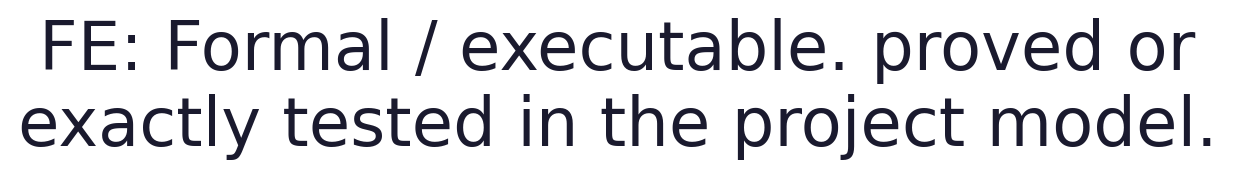
\includegraphics[keepaspectratio,width=0.98\linewidth,height=0.8\textheight,alt={FE: Formal / executable. proved or exactly tested in the project model.}]{../figures/evidence_replication_map.slide-class-formal-executable.png}
\refstepcounter{figure}\label{fig:evidence-replication-map-slide-panel-1}
\end{figure}
\end{frame}

\begin{frame}{Evidence classes and\ldots{} (part 7)}
\begin{figure}
\centering

\includegraphics[keepaspectratio,width=0.98\linewidth,height=0.8\textheight,alt={SC: Source-conditional. inherits only under the cited paper\textquotesingle s assumptions.}]{../figures/evidence_replication_map.slide-class-source-conditional.png}
\refstepcounter{figure}\label{fig:evidence-replication-map-slide-panel-2}
\end{figure}
\end{frame}

\begin{frame}{Evidence classes and\ldots{} (part 8)}
\begin{figure}
\centering

\includegraphics[keepaspectratio,width=0.98\linewidth,height=0.8\textheight,alt={CE: Conditional empirical. estimated in the declared finite design.}]{../figures/evidence_replication_map.slide-class-conditional-empirical.png}
\refstepcounter{figure}\label{fig:evidence-replication-map-slide-panel-3}
\end{figure}
\end{frame}

\begin{frame}{Evidence classes and\ldots{} (part 9)}
\begin{figure}
\centering

\includegraphics[keepaspectratio,width=0.98\linewidth,height=0.8\textheight,alt={SI: Scoped implementation. checks one software or protocol boundary.}]{../figures/evidence_replication_map.slide-class-scoped-implementation.png}
\refstepcounter{figure}\label{fig:evidence-replication-map-slide-panel-4}
\end{figure}
\end{frame}

\begin{frame}{Evidence classes and\ldots{} (part 10)}
\begin{figure}
\centering

\includegraphics[keepaspectratio,width=0.98\linewidth,height=0.8\textheight,alt={O: Open. not established by the current evidence.}]{../figures/evidence_replication_map.slide-class-open.png}
\refstepcounter{figure}\label{fig:evidence-replication-map-slide-panel-5}
\end{figure}
\end{frame}

\begin{frame}{Evidence classes and\ldots{} (part 11)}
\begin{figure}
\centering
\includegraphics[keepaspectratio,width=0.98\linewidth,height=0.8\textheight,alt={1. Project identity at c=0 {[}FE{]}
Estimand / unit: paired outputs {[}categorical posterior{]}}]{../figures/evidence_replication_map.slide-lane-1-estimand.png}
\refstepcounter{figure}\label{fig:evidence-replication-map-slide-panel-6}
\end{figure}
\end{frame}

\begin{frame}{Evidence classes and\ldots{} (part 12)}
\begin{figure}
\centering
\includegraphics[keepaspectratio,width=0.98\linewidth,height=0.8\textheight,alt={1. Project identity at c=0 {[}FE{]}
Independent unit: exact identity. Nesting: input \texorpdfstring{\ensuremath{\to}}{->} paired functions}]{../figures/evidence_replication_map.slide-lane-1-replication.png}
\refstepcounter{figure}\label{fig:evidence-replication-map-slide-panel-7}
\end{figure}
\end{frame}

\begin{frame}{Evidence classes and\ldots{} (part 13)}
\begin{figure}
\centering
\includegraphics[keepaspectratio,width=0.98\linewidth,height=0.8\textheight,alt={1. Project identity at c=0 {[}FE{]}
May support: project limit. Does not support: full source protocol}]{../figures/evidence_replication_map.slide-lane-1-claims.png}
\refstepcounter{figure}\label{fig:evidence-replication-map-slide-panel-8}
\end{figure}
\end{frame}

\begin{frame}{Evidence classes and\ldots{} (part 14)}
\begin{figure}
\centering
\includegraphics[keepaspectratio,width=0.98\linewidth,height=0.8\textheight,alt={2. Client-loss robustness {[}SC{]}
Estimand / unit: generalized posterior {[}client update{]}}]{../figures/evidence_replication_map.slide-lane-2-estimand.png}
\refstepcounter{figure}\label{fig:evidence-replication-map-slide-panel-9}
\end{figure}
\end{frame}

\begin{frame}{Evidence classes and\ldots{} (part 15)}
\begin{figure}
\centering
\includegraphics[keepaspectratio,width=0.98\linewidth,height=0.8\textheight,alt={2. Client-loss robustness {[}SC{]}
Independent unit: theorem; no empirical unit. Nesting: assumptions \texorpdfstring{\ensuremath{\to}}{->} update \texorpdfstring{\ensuremath{\to}}{->} posterior}]{../figures/evidence_replication_map.slide-lane-2-replication.png}
\refstepcounter{figure}\label{fig:evidence-replication-map-slide-panel-10}
\end{figure}
\end{frame}

\begin{frame}{Evidence classes and\ldots{} (part 16)}
\begin{figure}
\centering
\includegraphics[keepaspectratio,width=0.98\linewidth,height=0.8\textheight,alt={2. Client-loss robustness {[}SC{]}
May support: source theorem. Does not support: server theorem; performance; calibration}]{../figures/evidence_replication_map.slide-lane-2-claims.png}
\refstepcounter{figure}\label{fig:evidence-replication-map-slide-panel-11}
\end{figure}
\end{frame}

\begin{frame}{Evidence classes and\ldots{} (part 17)}
\begin{figure}
\centering
\includegraphics[keepaspectratio,width=0.98\linewidth,height=0.8\textheight,alt={3. Paired free-energy contrast {[}CE{]}
Estimand / unit: isolated - shared colony F {[}nats{]}}]{../figures/evidence_replication_map.slide-lane-3-estimand.png}
\refstepcounter{figure}\label{fig:evidence-replication-map-slide-panel-12}
\end{figure}
\end{frame}

\begin{frame}{Evidence classes and\ldots{} (part 18)}
\begin{figure}
\centering
\includegraphics[keepaspectratio,width=0.98\linewidth,height=0.8\textheight,alt={3. Paired free-energy contrast {[}CE{]}
Independent unit: configured seed. Nesting: study \texorpdfstring{\ensuremath{\to}}{->} seed \texorpdfstring{\ensuremath{\to}}{->} condition \texorpdfstring{\ensuremath{\to}}{->} agents}]{../figures/evidence_replication_map.slide-lane-3-replication.png}
\refstepcounter{figure}\label{fig:evidence-replication-map-slide-panel-13}
\end{figure}
\end{frame}

\begin{frame}{Evidence classes and\ldots{} (part 19)}
\begin{figure}
\centering
\includegraphics[keepaspectratio,width=0.98\linewidth,height=0.8\textheight,alt={3. Paired free-energy contrast {[}CE{]}
May support: paired protocol contrast. Does not support: general benefit; exact replication}]{../figures/evidence_replication_map.slide-lane-3-claims.png}
\refstepcounter{figure}\label{fig:evidence-replication-map-slide-panel-14}
\end{figure}
\end{frame}

\begin{frame}{Evidence classes and\ldots{} (part 20)}
\begin{figure}
\centering
\includegraphics[keepaspectratio,width=0.98\linewidth,height=0.8\textheight,alt={4. Dirichlet likelihood learning {[}CE{]}
Estimand / unit: KL(true A \textbar\textbar{} learned A) {[}nats{]}}]{../figures/evidence_replication_map.slide-lane-4-estimand.png}
\refstepcounter{figure}\label{fig:evidence-replication-map-slide-panel-15}
\end{figure}
\end{frame}

\begin{frame}{Evidence classes and\ldots{} (part 21)}
\begin{figure}
\centering
\includegraphics[keepaspectratio,width=0.98\linewidth,height=0.8\textheight,alt={4. Dirichlet likelihood learning {[}CE{]}
Independent unit: configured seed. Nesting: study \texorpdfstring{\ensuremath{\to}}{->} seed \texorpdfstring{\ensuremath{\to}}{->} steps \texorpdfstring{\ensuremath{\to}}{->} A rows}]{../figures/evidence_replication_map.slide-lane-4-replication.png}
\refstepcounter{figure}\label{fig:evidence-replication-map-slide-panel-16}
\end{figure}
\end{frame}

\begin{frame}{Evidence classes and\ldots{} (part 22)}
\begin{figure}
\centering
\includegraphics[keepaspectratio,width=0.98\linewidth,height=0.8\textheight,alt={4. Dirichlet likelihood learning {[}CE{]}
May support: executed conjugate path. Does not support: universal rate; continuous model}]{../figures/evidence_replication_map.slide-lane-4-claims.png}
\refstepcounter{figure}\label{fig:evidence-replication-map-slide-panel-17}
\end{figure}
\end{frame}

\begin{frame}{Evidence classes and\ldots{} (part 23)}
\begin{figure}
\centering
\includegraphics[keepaspectratio,width=0.98\linewidth,height=0.8\textheight,alt={5. Configured BMR sign control {[}FE{]}
Estimand / unit: pruning delta F {[}nats{]}}]{../figures/evidence_replication_map.slide-lane-5-estimand.png}
\refstepcounter{figure}\label{fig:evidence-replication-map-slide-panel-18}
\end{figure}
\end{frame}

\begin{frame}{Evidence classes and\ldots{} (part 24)}
\begin{figure}
\centering
\includegraphics[keepaspectratio,width=0.98\linewidth,height=0.8\textheight,alt={5. Configured BMR sign control {[}FE{]}
Independent unit: closed-form comparison. Nesting: posterior \texorpdfstring{\ensuremath{\to}}{->} pruning \texorpdfstring{\ensuremath{\to}}{->} signed delta}]{../figures/evidence_replication_map.slide-lane-5-replication.png}
\refstepcounter{figure}\label{fig:evidence-replication-map-slide-panel-19}
\end{figure}
\end{frame}

\begin{frame}{Evidence classes and\ldots{} (part 25)}
\begin{figure}
\centering
\includegraphics[keepaspectratio,width=0.98\linewidth,height=0.8\textheight,alt={5. Configured BMR sign control {[}FE{]}
May support: configured sign control. Does not support: universal emergence}]{../figures/evidence_replication_map.slide-lane-5-claims.png}
\refstepcounter{figure}\label{fig:evidence-replication-map-slide-panel-20}
\end{figure}
\end{frame}

\begin{frame}{Evidence classes and\ldots{} (part 26)}
\begin{figure}
\centering
\includegraphics[keepaspectratio,width=0.98\linewidth,height=0.8\textheight,alt={6. Exploratory client baseline {[}CE{]}
Estimand / unit: joint-config accuracy {[}fraction{]}}]{../figures/evidence_replication_map.slide-lane-6-estimand.png}
\refstepcounter{figure}\label{fig:evidence-replication-map-slide-panel-21}
\end{figure}
\end{frame}

\begin{frame}{Evidence classes and\ldots{} (part 27)}
\begin{figure}
\centering
\includegraphics[keepaspectratio,width=0.98\linewidth,height=0.8\textheight,alt={6. Exploratory client baseline {[}CE{]}
Independent unit: synthetic seed. Nesting: sweep \texorpdfstring{\ensuremath{\to}}{->} seed \texorpdfstring{\ensuremath{\to}}{->} client \texorpdfstring{\ensuremath{\to}}{->} row}]{../figures/evidence_replication_map.slide-lane-6-replication.png}
\refstepcounter{figure}\label{fig:evidence-replication-map-slide-panel-22}
\end{figure}
\end{frame}

\begin{frame}{Evidence classes and\ldots{} (part 28)}
\begin{figure}
\centering
\includegraphics[keepaspectratio,width=0.98\linewidth,height=0.8\textheight,alt={6. Exploratory client baseline {[}CE{]}
May support: composite configuration contrast. Does not support: RCCE-only; calibration; BNN claims}]{../figures/evidence_replication_map.slide-lane-6-claims.png}
\refstepcounter{figure}\label{fig:evidence-replication-map-slide-panel-23}
\end{figure}
\end{frame}

\begin{frame}{Evidence classes and\ldots{} (part 29)}
\begin{figure}
\centering
\includegraphics[keepaspectratio,width=0.98\linewidth,height=0.8\textheight,alt={7. Server reweighting heuristic {[}CE{]}
Estimand / unit: robust - naive {[}p or fraction{]}}]{../figures/evidence_replication_map.slide-lane-7-estimand.png}
\refstepcounter{figure}\label{fig:evidence-replication-map-slide-panel-24}
\end{figure}
\end{frame}

\begin{frame}{Evidence classes and\ldots{} (part 30)}
\begin{figure}
\centering
\includegraphics[keepaspectratio,width=0.98\linewidth,height=0.8\textheight,alt={7. Server reweighting heuristic {[}CE{]}
Independent unit: seed or matched trial. Nesting: study \texorpdfstring{\ensuremath{\to}}{->} seed/world \texorpdfstring{\ensuremath{\to}}{->} trial \texorpdfstring{\ensuremath{\to}}{->} agents}]{../figures/evidence_replication_map.slide-lane-7-replication.png}
\refstepcounter{figure}\label{fig:evidence-replication-map-slide-panel-25}
\end{figure}
\end{frame}

\begin{frame}{Evidence classes and\ldots{} (part 31)}
\begin{figure}
\centering
\includegraphics[keepaspectratio,width=0.98\linewidth,height=0.8\textheight,alt={7. Server reweighting heuristic {[}CE{]}
May support: finite mechanism behavior. Does not support: influence bound; Byzantine tol.; universal win}]{../figures/evidence_replication_map.slide-lane-7-claims.png}
\refstepcounter{figure}\label{fig:evidence-replication-map-slide-panel-26}
\end{figure}
\end{frame}

\begin{frame}{Evidence classes and\ldots{} (part 32)}
\begin{figure}
\centering
\includegraphics[keepaspectratio,width=0.98\linewidth,height=0.8\textheight,alt={8. Variational server rule {[}FE{]}
Estimand / unit: descent, weights, transfer {[}mixed{]}}]{../figures/evidence_replication_map.slide-lane-8-estimand.png}
\refstepcounter{figure}\label{fig:evidence-replication-map-slide-panel-27}
\end{figure}
\end{frame}

\begin{frame}{Evidence classes and\ldots{} (part 33)}
\begin{figure}
\centering
\includegraphics[keepaspectratio,width=0.98\linewidth,height=0.8\textheight,alt={8. Variational server rule {[}FE{]}
Independent unit: identity or seeded path. Nesting: config \texorpdfstring{\ensuremath{\to}}{->} start \texorpdfstring{\ensuremath{\to}}{->} iterates}]{../figures/evidence_replication_map.slide-lane-8-replication.png}
\refstepcounter{figure}\label{fig:evidence-replication-map-slide-panel-28}
\end{figure}
\end{frame}

\begin{frame}{Evidence classes and\ldots{} (part 34)}
\begin{figure}
\centering
\includegraphics[keepaspectratio,width=0.98\linewidth,height=0.8\textheight,alt={8. Variational server rule {[}FE{]}
May support: objective + tested transfer. Does not support: global or universal claim}]{../figures/evidence_replication_map.slide-lane-8-claims.png}
\refstepcounter{figure}\label{fig:evidence-replication-map-slide-panel-29}
\end{figure}
\end{frame}

\begin{frame}{Evidence classes and\ldots{} (part 35)}
\begin{figure}
\centering
\includegraphics[keepaspectratio,width=0.98\linewidth,height=0.8\textheight,alt={9. Moving / disjoint-FOV contrasts {[}CE{]}
Estimand / unit: policy/sharing {[}fraction, nats, steps{]}}]{../figures/evidence_replication_map.slide-lane-9-estimand.png}
\refstepcounter{figure}\label{fig:evidence-replication-map-slide-panel-30}
\end{figure}
\end{frame}

\begin{frame}{Evidence classes and\ldots{} (part 36)}
\begin{figure}
\centering
\includegraphics[keepaspectratio,width=0.98\linewidth,height=0.8\textheight,alt={9. Moving / disjoint-FOV contrasts {[}CE{]}
Independent unit: seed or fixed world. Nesting: world \texorpdfstring{\ensuremath{\to}}{->} seed \texorpdfstring{\ensuremath{\to}}{->} condition \texorpdfstring{\ensuremath{\to}}{->} agents/steps}]{../figures/evidence_replication_map.slide-lane-9-replication.png}
\refstepcounter{figure}\label{fig:evidence-replication-map-slide-panel-31}
\end{figure}
\end{frame}

\begin{frame}{Evidence classes and\ldots{} (part 37)}
\begin{figure}
\centering
\includegraphics[keepaspectratio,width=0.98\linewidth,height=0.8\textheight,alt={9. Moving / disjoint-FOV contrasts {[}CE{]}
May support: executed-world behavior. Does not support: universal claim; physical multi-host}]{../figures/evidence_replication_map.slide-lane-9-claims.png}
\refstepcounter{figure}\label{fig:evidence-replication-map-slide-panel-32}
\end{figure}
\end{frame}

\begin{frame}{Evidence classes and\ldots{} (part 38)}
\begin{figure}
\centering
\includegraphics[keepaspectratio,width=0.98\linewidth,height=0.8\textheight,alt={10. Hierarchy / sensitivity diagnostics {[}CE{]}
Estimand / unit: posterior/gap/gate {[}probability, fraction, nats{]}}]{../figures/evidence_replication_map.slide-lane-10-estimand.png}
\refstepcounter{figure}\label{fig:evidence-replication-map-slide-panel-33}
\end{figure}
\end{frame}

\begin{frame}{Evidence classes and\ldots{} (part 39)}
\begin{figure}
\centering
\includegraphics[keepaspectratio,width=0.98\linewidth,height=0.8\textheight,alt={10. Hierarchy / sensitivity diagnostics {[}CE{]}
Independent unit: seed or fixed diagnostic. Nesting: world \texorpdfstring{\ensuremath{\to}}{->} seed \texorpdfstring{\ensuremath{\to}}{->} level \texorpdfstring{\ensuremath{\to}}{->} agents/states}]{../figures/evidence_replication_map.slide-lane-10-replication.png}
\refstepcounter{figure}\label{fig:evidence-replication-map-slide-panel-34}
\end{figure}
\end{frame}

\begin{frame}{Evidence classes and\ldots{} (part 40)}
\begin{figure}
\centering
\includegraphics[keepaspectratio,width=0.98\linewidth,height=0.8\textheight,alt={10. Hierarchy / sensitivity diagnostics {[}CE{]}
May support: executed hierarchy design. Does not support: universal benefit, depth, or emergence}]{../figures/evidence_replication_map.slide-lane-10-claims.png}
\refstepcounter{figure}\label{fig:evidence-replication-map-slide-panel-35}
\end{figure}
\end{frame}

\begin{frame}{Evidence classes and\ldots{} (part 41)}
\begin{figure}
\centering
\includegraphics[keepaspectratio,width=0.98\linewidth,height=0.8\textheight,alt={11. Acuity recovery diagnostic {[}CE{]}
Estimand / unit: acuity, error, R² {[}p or unitless{]}}]{../figures/evidence_replication_map.slide-lane-11-estimand.png}
\refstepcounter{figure}\label{fig:evidence-replication-map-slide-panel-36}
\end{figure}
\end{frame}

\begin{frame}{Evidence classes and\ldots{} (part 42)}
\begin{figure}
\centering
\includegraphics[keepaspectratio,width=0.98\linewidth,height=0.8\textheight,alt={11. Acuity recovery diagnostic {[}CE{]}
Independent unit: trial within acuity cell. Nesting: grid point \texorpdfstring{\ensuremath{\to}}{->} trial \texorpdfstring{\ensuremath{\to}}{->} rows \texorpdfstring{\ensuremath{\to}}{->} estimate}]{../figures/evidence_replication_map.slide-lane-11-replication.png}
\refstepcounter{figure}\label{fig:evidence-replication-map-slide-panel-37}
\end{figure}
\end{frame}

\begin{frame}{Evidence classes and\ldots{} (part 43)}
\begin{figure}
\centering
\includegraphics[keepaspectratio,width=0.98\linewidth,height=0.8\textheight,alt={11. Acuity recovery diagnostic {[}CE{]}
May support: finite-grid recovery. Does not support: global structural identifiability}]{../figures/evidence_replication_map.slide-lane-11-claims.png}
\refstepcounter{figure}\label{fig:evidence-replication-map-slide-panel-38}
\end{figure}
\end{frame}

\begin{frame}{Evidence classes and\ldots{} (part 44)}
\begin{figure}
\centering
\includegraphics[keepaspectratio,width=0.98\linewidth,height=0.8\textheight,alt={12. Protocol-v1 / replay integrity {[}SI{]}
Estimand / unit: frame/replay match {[}frame or round{]}}]{../figures/evidence_replication_map.slide-lane-12-estimand.png}
\refstepcounter{figure}\label{fig:evidence-replication-map-slide-panel-39}
\end{figure}
\end{frame}

\begin{frame}{Evidence classes and\ldots{} (part 45)}
\begin{figure}
\centering
\includegraphics[keepaspectratio,width=0.98\linewidth,height=0.8\textheight,alt={12. Protocol-v1 / replay integrity {[}SI{]}
Independent unit: local round. Nesting: round \texorpdfstring{\ensuremath{\to}}{->} workers \texorpdfstring{\ensuremath{\to}}{->} frames \texorpdfstring{\ensuremath{\to}}{->} fields}]{../figures/evidence_replication_map.slide-lane-12-replication.png}
\refstepcounter{figure}\label{fig:evidence-replication-map-slide-panel-40}
\end{figure}
\end{frame}

\begin{frame}{Evidence classes and\ldots{} (part 46)}
\begin{figure}
\centering
\includegraphics[keepaspectratio,width=0.98\linewidth,height=0.8\textheight,alt={12. Protocol-v1 / replay integrity {[}SI{]}
May support: protocol-v1 local integrity. Does not support: encryption/mTLS; multi-host; Byzantine tol.}]{../figures/evidence_replication_map.slide-lane-12-claims.png}
\refstepcounter{figure}\label{fig:evidence-replication-map-slide-panel-41}
\end{figure}
\end{frame}

\begin{frame}{Evidence classes and\ldots{} (part 47)}
\begin{figure}
\centering
\includegraphics[keepaspectratio,width=0.98\linewidth,height=0.8\textheight,alt={13. Application receipt {[}SI{]}
Estimand / unit: hash/source agreement {[}artifact{]}}]{../figures/evidence_replication_map.slide-lane-13-estimand.png}
\refstepcounter{figure}\label{fig:evidence-replication-map-slide-panel-42}
\end{figure}
\end{frame}

\begin{frame}{Evidence classes and\ldots{} (part 48)}
\begin{figure}
\centering
\includegraphics[keepaspectratio,width=0.98\linewidth,height=0.8\textheight,alt={13. Application receipt {[}SI{]}
Independent unit: application invocation. Nesting: invocation \texorpdfstring{\ensuremath{\to}}{->} artifacts \texorpdfstring{\ensuremath{\to}}{->} levels}]{../figures/evidence_replication_map.slide-lane-13-replication.png}
\refstepcounter{figure}\label{fig:evidence-replication-map-slide-panel-43}
\end{figure}
\end{frame}

\begin{frame}{Evidence classes and\ldots{} (part 49)}
\begin{figure}
\centering
\includegraphics[keepaspectratio,width=0.98\linewidth,height=0.8\textheight,alt={13. Application receipt {[}SI{]}
May support: hashes; requested source match. Does not support: validity; decision; acceptance}]{../figures/evidence_replication_map.slide-lane-13-claims.png}
\refstepcounter{figure}\label{fig:evidence-replication-map-slide-panel-44}
\end{figure}
\end{frame}

\begin{frame}{Evidence classes and\ldots{} (part 50)}
\begin{figure}
\centering
\includegraphics[keepaspectratio,width=0.98\linewidth,height=0.8\textheight,alt={14. External calibration / confirmation {[}O{]}
Estimand / unit: paired log score {[}nats/observation{]}}]{../figures/evidence_replication_map.slide-lane-14-estimand.png}
\refstepcounter{figure}\label{fig:evidence-replication-map-slide-panel-45}
\end{figure}
\end{frame}

\begin{frame}{Evidence classes and\ldots{} (part 51)}
\begin{figure}
\centering
\includegraphics[keepaspectratio,width=0.98\linewidth,height=0.8\textheight,alt={14. External calibration / confirmation {[}O{]}
Independent unit: dataset highest; seeds nested. Nesting: dataset \texorpdfstring{\ensuremath{\to}}{->} seed \texorpdfstring{\ensuremath{\to}}{->} clients \texorpdfstring{\ensuremath{\to}}{->} rows}]{../figures/evidence_replication_map.slide-lane-14-replication.png}
\refstepcounter{figure}\label{fig:evidence-replication-map-slide-panel-46}
\end{figure}
\end{frame}

\begin{frame}{Evidence classes and\ldots{} (part 52)}
\begin{figure}
\centering
\includegraphics[keepaspectratio,width=0.98\linewidth,height=0.8\textheight,alt={14. External calibration / confirmation {[}O{]}
May support: none before design + report. Does not support: retrospective or pooled-dataset claim}]{../figures/evidence_replication_map.slide-lane-14-claims.png}
\refstepcounter{figure}\label{fig:evidence-replication-map-slide-panel-47}
\end{figure}
\end{frame}

\begin{frame}{Evidence classes and\ldots{} (part 53)}
\begin{figure}
\centering
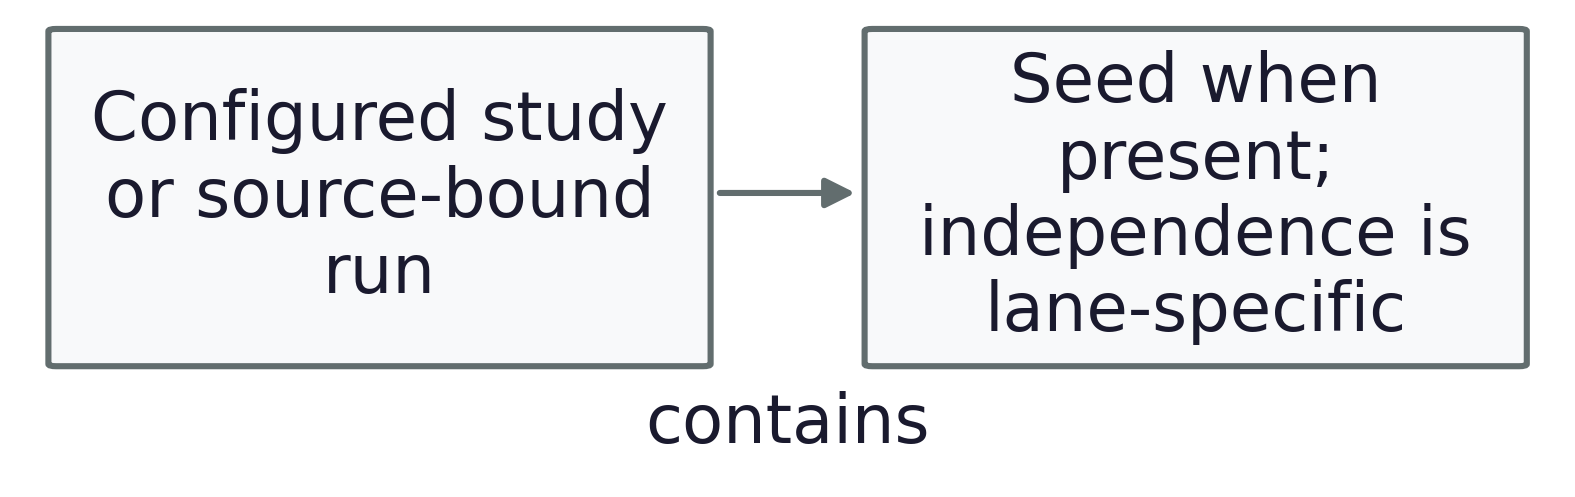
\includegraphics[keepaspectratio,width=0.98\linewidth,height=0.8\textheight,alt={Configured study or source-bound run → Seed when present; independence is lane-specific: contains; nesting.}]{../figures/evidence_replication_map.slide-nesting-1.png}
\refstepcounter{figure}\label{fig:evidence-replication-map-slide-panel-48}
\end{figure}
\end{frame}

\begin{frame}{Evidence classes and\ldots{} (part 54)}
\begin{figure}
\centering
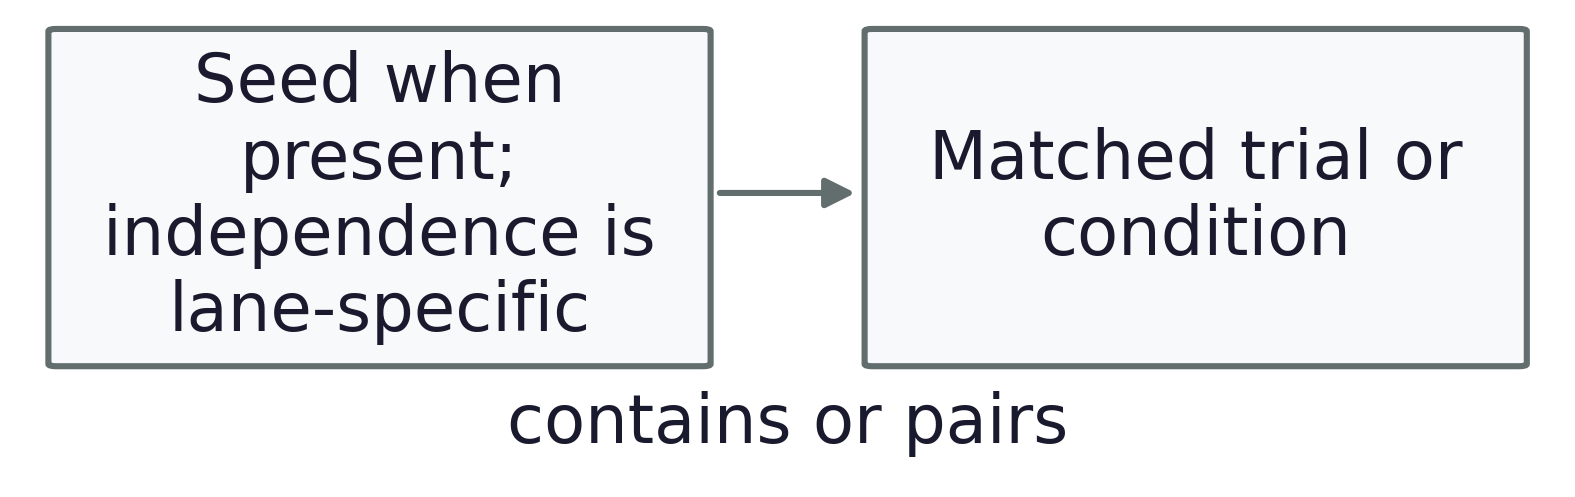
\includegraphics[keepaspectratio,width=0.98\linewidth,height=0.8\textheight,alt={Seed when present; independence is lane-specific → Matched trial or condition: contains or pairs; nesting.}]{../figures/evidence_replication_map.slide-nesting-2.png}
\refstepcounter{figure}\label{fig:evidence-replication-map-slide-panel-49}
\end{figure}
\end{frame}

\begin{frame}{Evidence classes and\ldots{} (part 55)}
\begin{figure}
\centering
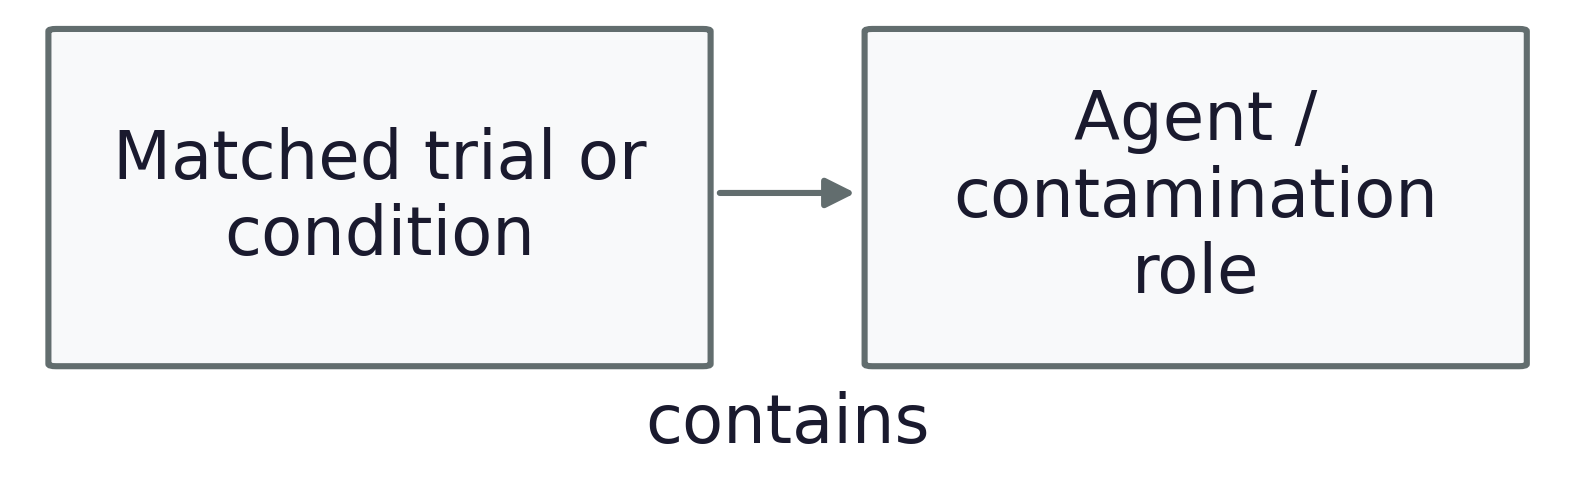
\includegraphics[keepaspectratio,width=0.98\linewidth,height=0.8\textheight,alt={Matched trial or condition → Agent / contamination role: contains; nesting.}]{../figures/evidence_replication_map.slide-nesting-3.png}
\refstepcounter{figure}\label{fig:evidence-replication-map-slide-panel-50}
\end{figure}
\end{frame}

\begin{frame}{Evidence classes and\ldots{} (part 56)}
\begin{figure}
\centering
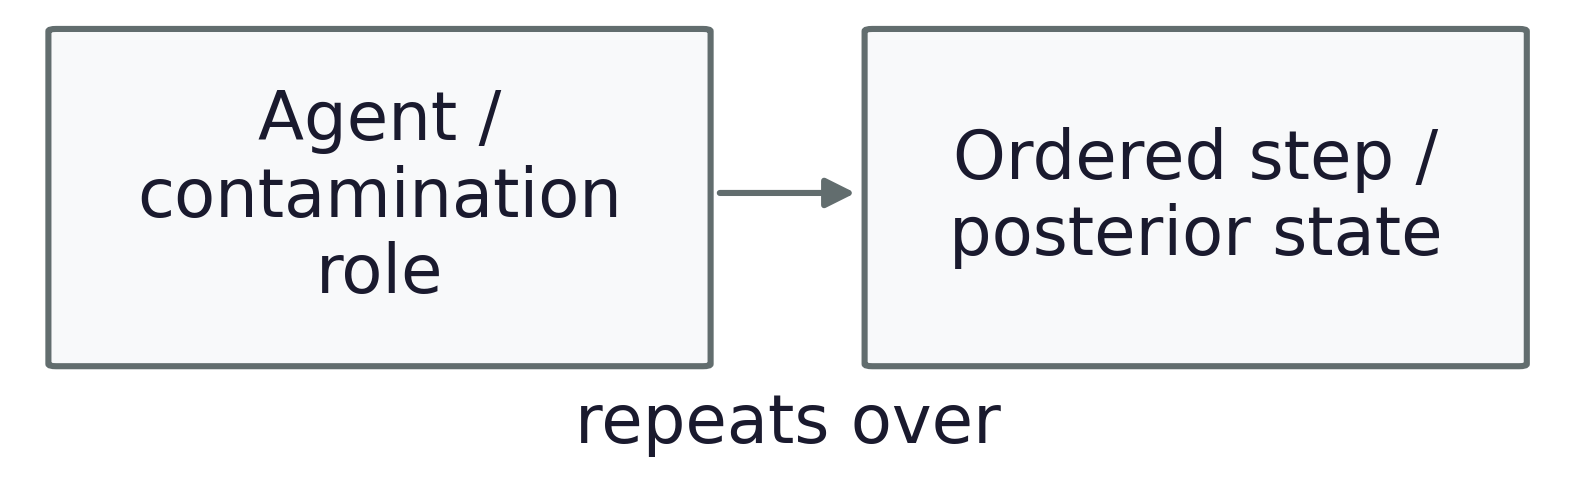
\includegraphics[keepaspectratio,width=0.98\linewidth,height=0.8\textheight,alt={Agent / contamination role → Ordered step / posterior state: repeats over; nesting.}]{../figures/evidence_replication_map.slide-nesting-4.png}
\refstepcounter{figure}\label{fig:evidence-replication-map-slide-panel-51}
\end{figure}
\end{frame}

\begin{frame}{Evidence classes and\ldots{} (part 57)}
\begin{figure}
\centering
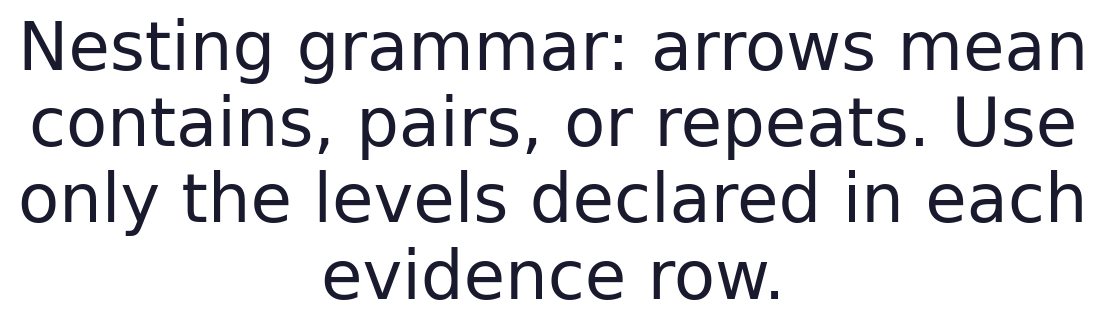
\includegraphics[keepaspectratio,width=0.98\linewidth,height=0.8\textheight,alt={Nesting grammar: arrows mean contains, pairs, or repeats. Use only the levels declared in each evidence row.}]{../figures/evidence_replication_map.slide-nesting-scope.png}
\refstepcounter{figure}\label{fig:evidence-replication-map-slide-panel-52}
\end{figure}
\end{frame}

\begin{frame}{Evidence classes and\ldots{} (part 58)}
\begin{figure}
\centering
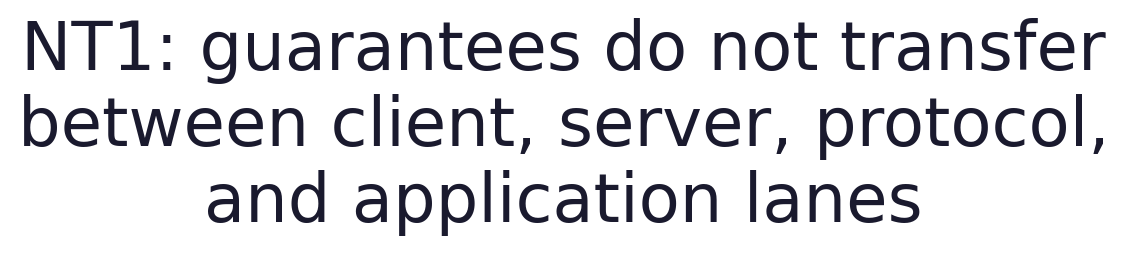
\includegraphics[keepaspectratio,width=0.98\linewidth,height=0.8\textheight,alt={NT1: guarantees do not transfer between client, server, protocol, and application lanes}]{../figures/evidence_replication_map.slide-no-transfer-1.png}
\refstepcounter{figure}\label{fig:evidence-replication-map-slide-panel-53}
\end{figure}
\end{frame}

\begin{frame}{Evidence classes and\ldots{} (part 59)}
\begin{figure}
\centering

\includegraphics[keepaspectratio,width=0.98\linewidth,height=0.8\textheight,alt={NT2: nested agents, trials, and time steps are not promoted to independent datasets}]{../figures/evidence_replication_map.slide-no-transfer-2.png}
\refstepcounter{figure}\label{fig:evidence-replication-map-slide-panel-54}
\end{figure}
\end{frame}

\begin{frame}{Evidence classes and\ldots{} (part 60)}
\begin{figure}
\centering
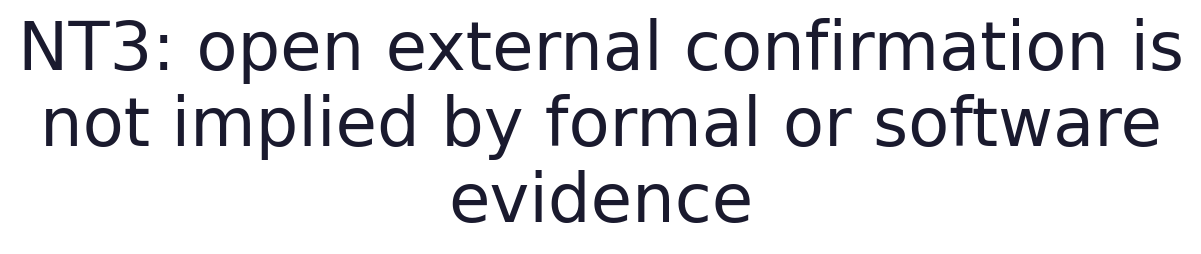
\includegraphics[keepaspectratio,width=0.98\linewidth,height=0.8\textheight,alt={NT3: open external confirmation is not implied by formal or software evidence}]{../figures/evidence_replication_map.slide-no-transfer-3.png}
\refstepcounter{figure}\label{fig:evidence-replication-map-slide-panel-55}
\end{figure}
\end{frame}

\begin{frame}{Computational complexity and scaling diagnostic}
\protect\phantomsection\label{sec:methods-complexity}
The release now reports computational complexity from the implementation
itself. Let \(N\) be the number of agents, \(S\) the number of
categorical states, \(I\) the solver-iteration budget, \(B\) the number
of variational starts,
\end{frame}

\begin{frame}{Computational complexity\ldots{} (part 2)}
and \(M\) the number of conditionally independent observation
modalities.
\end{frame}

\begin{frame}[fragile]{Computational complexity\ldots{} (part 3)}
The dominant dense work and the storage actually retained by the current
NumPy paths are summarized separately so neither quantity is compressed
at presentation scale. Here \texttt{LOO} means self-excluding
leave-one-out sharing, and \texttt{server\ round} excludes queue and
network wait.
\end{frame}

\begin{frame}{Computational complexity\ldots{} (part 4)}
\textbf{Time, aggregation.} The log, robust, and variational pools have
orders \(\Theta(N S)\), \(\Theta(I N S)\), and \(\Theta(B I N S)\),
respectively.
\end{frame}

\begin{frame}{Computational complexity\ldots{} (part 5)}
\textbf{Time, sharing and inference.} Naive LOO, robust LOO, state
inference, and a server round have orders \(\Theta(N^2 S)\),
\(\Theta(I N^2 S)\), \(\Theta(M S)\), and \(\Theta(N log N + I N S)\),
respectively.
\end{frame}

\begin{frame}{Computational complexity\ldots{} (part 6)}
\textbf{Storage, aggregation.} The log, robust, and variational pools
retain or peak at \(\Theta(N S)\), \(\Theta(N S + I S)\), and
\(\Theta(N S + I S + B S)\), respectively.
\end{frame}

\begin{frame}{Computational complexity\ldots{} (part 7)}
\textbf{Storage, sharing and inference.} Naive LOO, robust LOO, state
inference, and a server round retain or peak at \(\Theta(N S)\),
\(\Theta(N S + I S)\), \(\Theta(S)\), and \(\Theta(N S)\), respectively.
\end{frame}

\begin{frame}{Computational complexity\ldots{} (part 8)}
These are dominant interaction counts, not hardware-independent FLOP
totals. The \(N^2\) sharing term is material: with sensory attenuation
enabled, one round computes one global pool and one leave-one-out pool
per agent.
\end{frame}

\begin{frame}{Computational complexity\ldots{} (part 9)}
The iterative server rules additionally retain their returned
per-iteration histories, which is why their storage rows include
\(I S\). The server row includes worker-ID sorting and dense
aggregation; incoming serialized belief volume is linear in \(N S\),
\end{frame}

\begin{frame}{Computational complexity\ldots{} (part 10)}
while queue and network latency are deliberately outside this
local-compute accounting.
\end{frame}

\begin{frame}{Computational complexity\ldots{} (part 11)}
The local path serializes one consensus-plus-weight result; if physical
broadcast bytes are counted per recipient, that outgoing volume
additionally has an \(N^2\) term because each result carries the \(N\)
agent weights.
\end{frame}

\begin{frame}{Computational complexity\ldots{} (part 12)}
The accompanying seeded benchmark measures the real public call paths on
the declared grids \(N \in \{4, 8, 16, 32, 64\}\), \(S \in
\{256, 512, 1024, 2048, 4096\}\), self-excluding sharing \(N \in
\{4, 8, 16, 32\}\), and \(M \in
\{1, 2, 4, 8\}\).
\end{frame}

\begin{frame}{Computational complexity\ldots{} (part 13)}
The fixed dimensions are \(N=256\), \(S=64\) for aggregation, and
\(S=16384\) for state inference; direct aggregation and server timings
use \(I=6\), while the public robust self-excluding sharing path uses
its solver budget \(I=32\); the default variational path uses \(B=3\).
\end{frame}

\begin{frame}{Computational complexity\ldots{} (part 14)}
Each grid point is warmed up \(1\) time(s) and measured \(5\) time(s),
with median time plotted and the observed repeat range shown as a
min--max bar.

The fixed input seed is \(20260728\) on the \(arm64\) machine using
Python \(3.13.11\) and NumPy \(2.4.2\).
\end{frame}

\begin{frame}{Computational complexity\ldots{} (part 15)}
The measured log--log slopes are descriptive checks of the expected
orders, not performance guarantees: agent-axis slopes are 0.99
(log-linear), 0.94 (iterative robust), 0.79 (variational), 1.64 (naive
self-excluding sharing), and 1.93 (robust self-excluding sharing);
state-axis slopes are 0.96, 0.96, and 0.95;
\end{frame}

\begin{frame}{Computational complexity\ldots{} (part 16)}
the modality-axis inference slope is 0.66.

The slope fit is a timing diagnostic on this machine, not an inferential
test and not evidence that the same constants hold under another BLAS,
accelerator, process topology, or distributed network.
\end{frame}

\begin{frame}{Computational complexity\ldots{} (part 17)}
A finite grid can also yield a sublinear fitted slope when validation,
allocation, cache, and interpreter overheads are material; the
implementation-derived order is the governing claim, not equality
between a finite-grid slope and its exponent.
\end{frame}

\begin{frame}{Computational complexity\ldots{} (part 18)}
The timing plot in fig.~7 visualizes the
implementation-derived orders and the corresponding finite-grid timing
diagnostic.
\end{frame}

\begin{frame}{Computational complexity\ldots{} (part 19)}
\begin{figure}
\centering
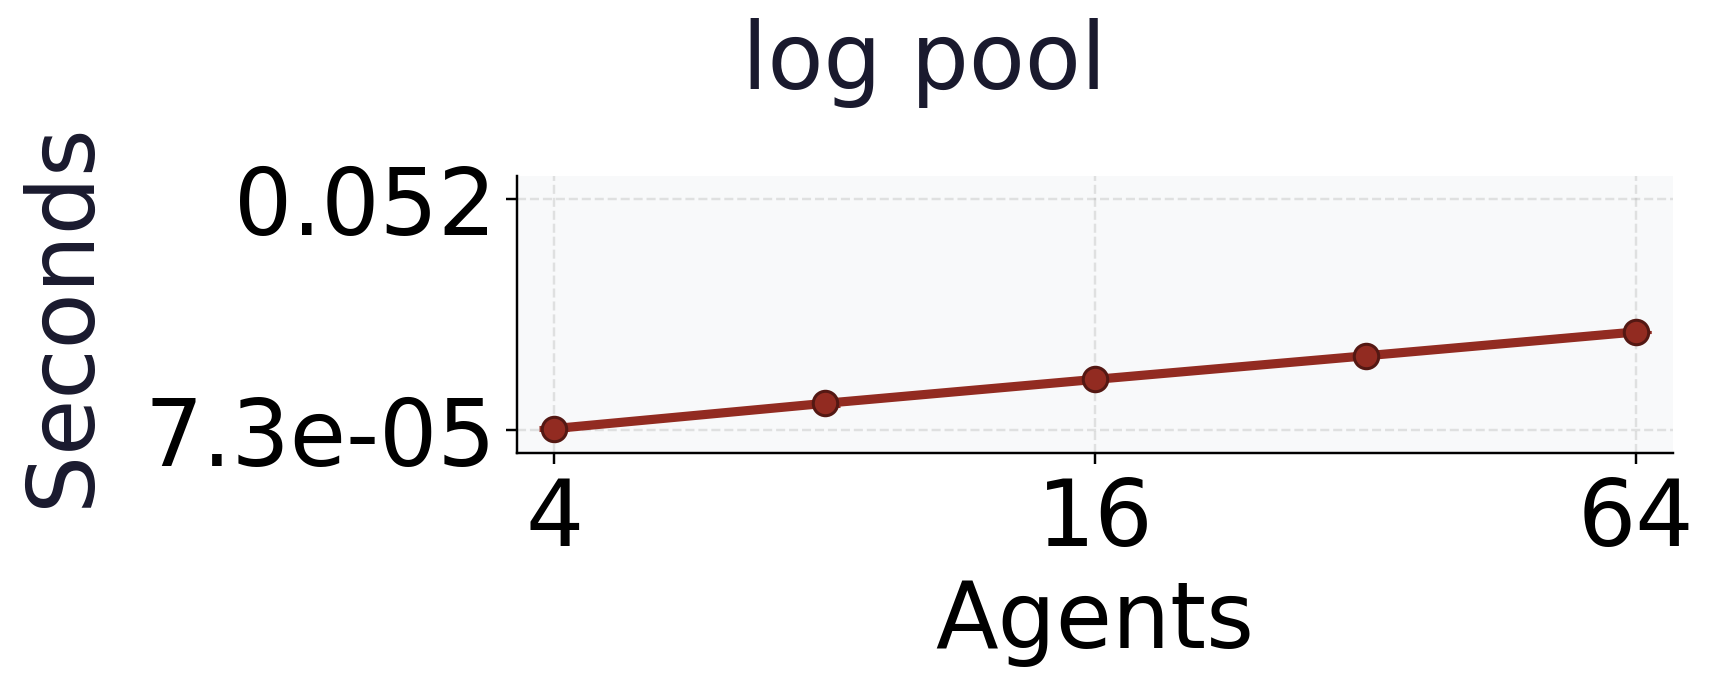
\includegraphics[keepaspectratio,width=0.98\linewidth,height=0.8\textheight,alt={log\_linear\_pool by agents: all measured medians, observed min-max ranges and normalized expected-exponent guide on common group scales.}]{../figures/complexity_scaling.slide-group-1-log-linear-pool.png}
\refstepcounter{figure}\label{fig:complexity-scaling-slide-panel-1}
\end{figure}
\end{frame}

\begin{frame}{Computational complexity\ldots{} (part 20)}
\begin{figure}
\centering
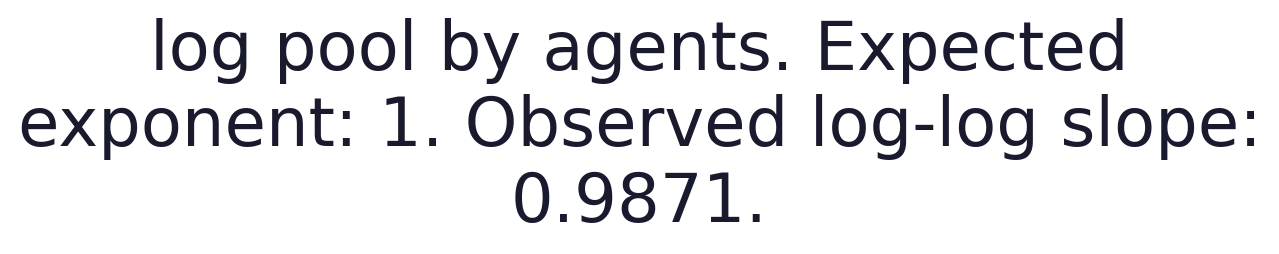
\includegraphics[keepaspectratio,width=0.98\linewidth,height=0.8\textheight,alt={log pool by agents. Expected exponent: 1. Observed log-log slope: 0.9871.}]{../figures/complexity_scaling.slide-group-1-log-linear-pool-guide.png}
\refstepcounter{figure}\label{fig:complexity-scaling-slide-panel-2}
\end{figure}
\end{frame}

\begin{frame}{Computational complexity\ldots{} (part 21)}
\begin{figure}
\centering
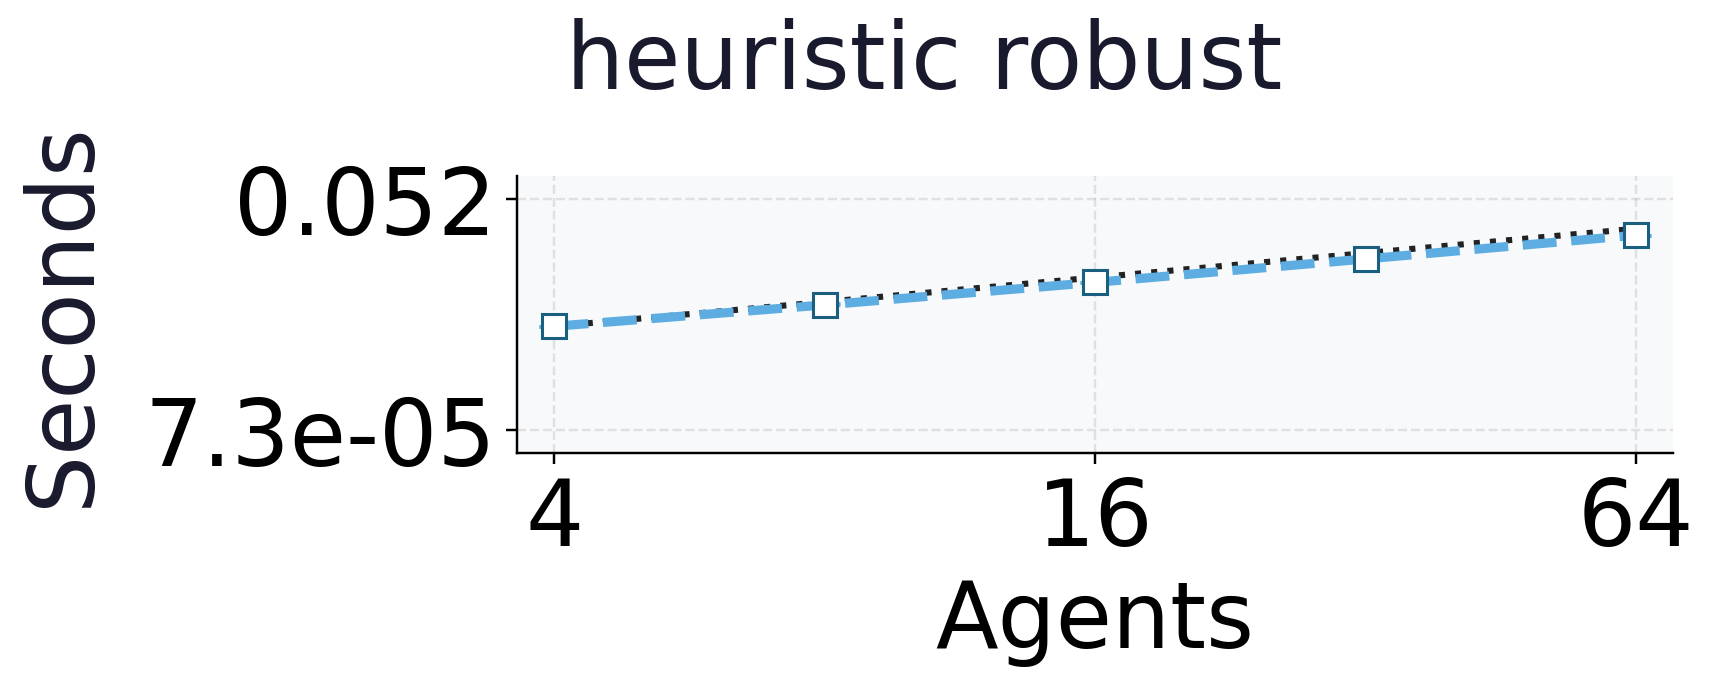
\includegraphics[keepaspectratio,width=0.98\linewidth,height=0.8\textheight,alt={robust\_aggregate by agents: all measured medians, observed min-max ranges and normalized expected-exponent guide on common group scales.}]{../figures/complexity_scaling.slide-group-1-robust-aggregate.png}
\refstepcounter{figure}\label{fig:complexity-scaling-slide-panel-3}
\end{figure}
\end{frame}

\begin{frame}{Computational complexity\ldots{} (part 22)}
\begin{figure}
\centering
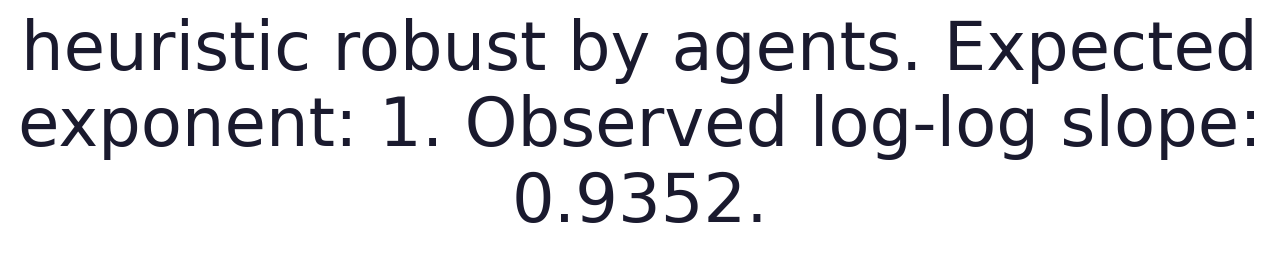
\includegraphics[keepaspectratio,width=0.98\linewidth,height=0.8\textheight,alt={heuristic robust by agents. Expected exponent: 1. Observed log-log slope: 0.9352.}]{../figures/complexity_scaling.slide-group-1-robust-aggregate-guide.png}
\refstepcounter{figure}\label{fig:complexity-scaling-slide-panel-4}
\end{figure}
\end{frame}

\begin{frame}{Computational complexity\ldots{} (part 23)}
\begin{figure}
\centering
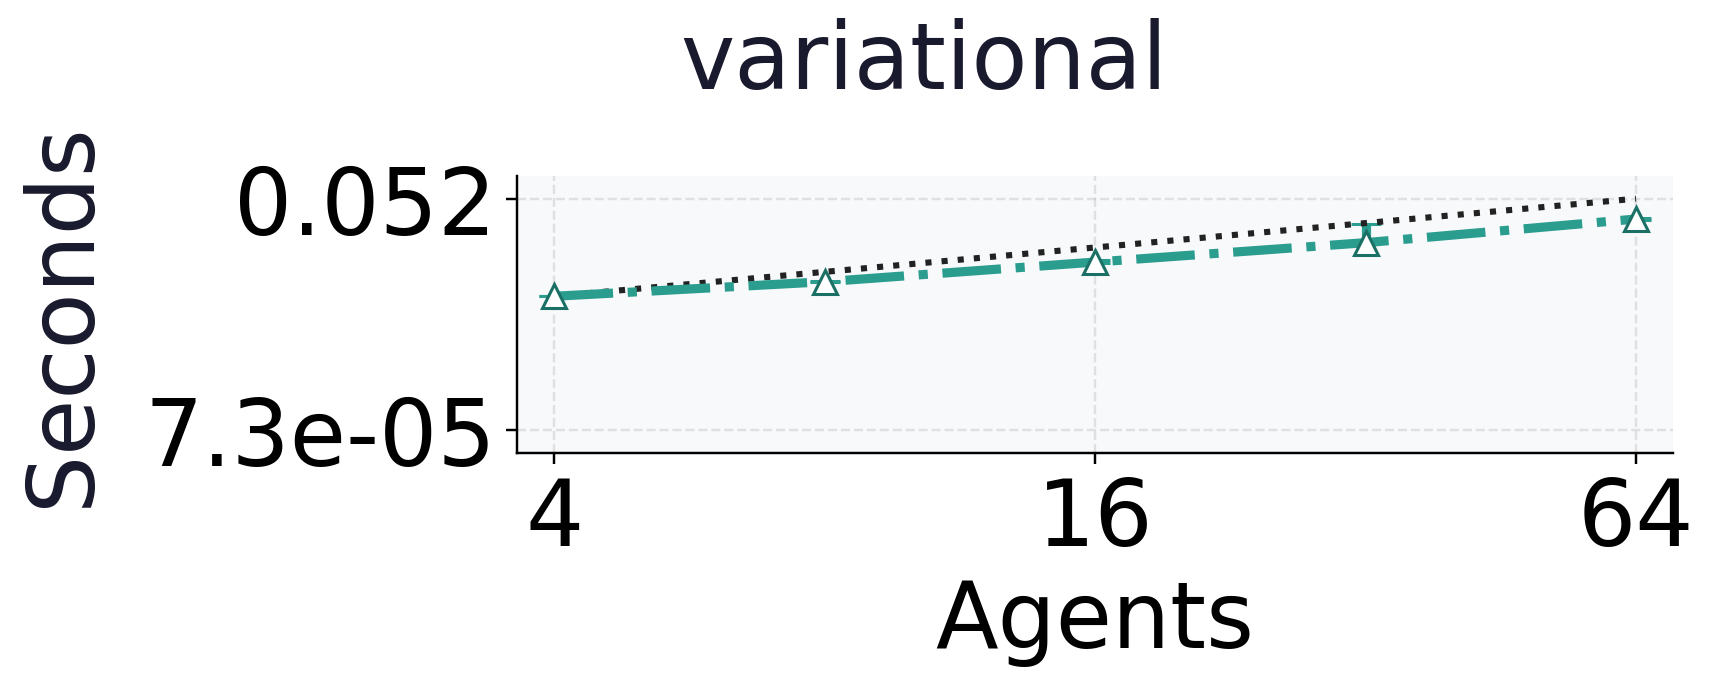
\includegraphics[keepaspectratio,width=0.98\linewidth,height=0.8\textheight,alt={variational\_aggregate by agents: all measured medians, observed min-max ranges and normalized expected-exponent guide on common group scales.}]{../figures/complexity_scaling.slide-group-1-variational-aggregate.png}
\refstepcounter{figure}\label{fig:complexity-scaling-slide-panel-5}
\end{figure}
\end{frame}

\begin{frame}{Computational complexity\ldots{} (part 24)}
\begin{figure}
\centering
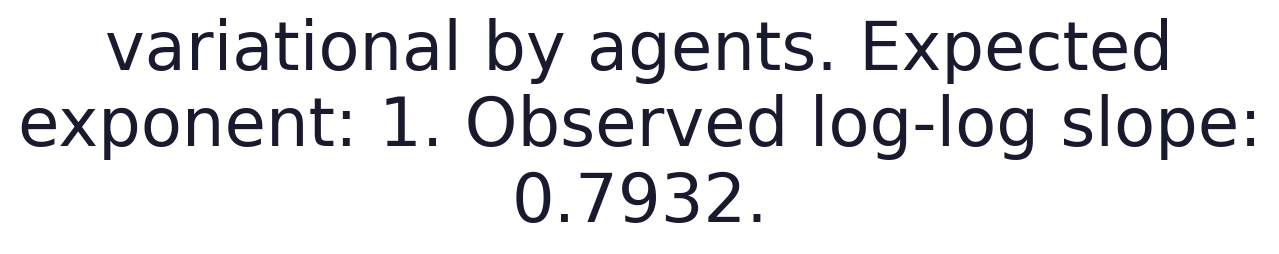
\includegraphics[keepaspectratio,width=0.98\linewidth,height=0.8\textheight,alt={variational by agents. Expected exponent: 1. Observed log-log slope: 0.7932.}]{../figures/complexity_scaling.slide-group-1-variational-aggregate-guide.png}
\refstepcounter{figure}\label{fig:complexity-scaling-slide-panel-6}
\end{figure}
\end{frame}

\begin{frame}{Computational complexity\ldots{} (part 25)}
\begin{figure}
\centering
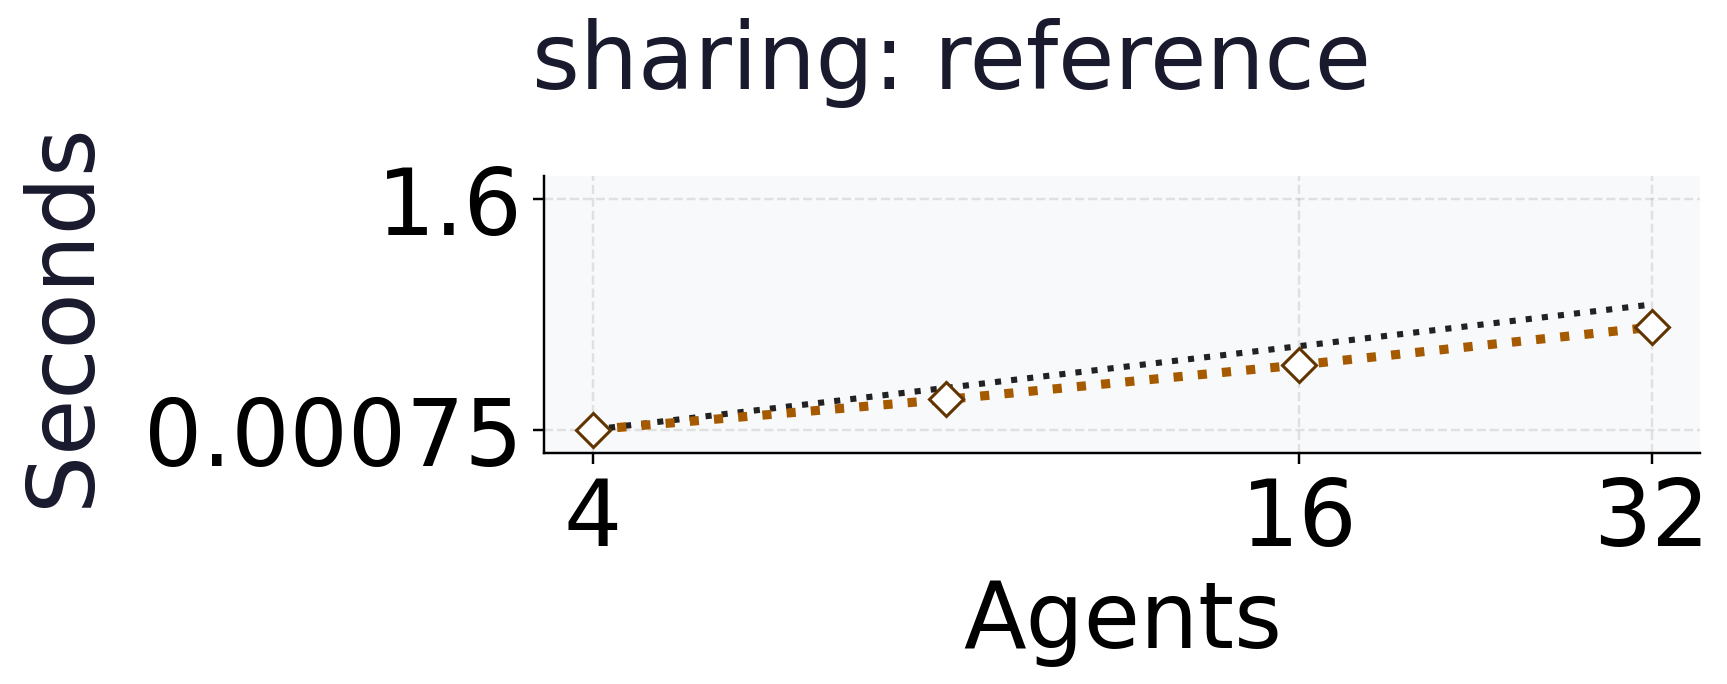
\includegraphics[keepaspectratio,width=0.98\linewidth,height=0.8\textheight,alt={share\_round\_naive by agents: all measured medians, observed min-max ranges and normalized expected-exponent guide on common group scales.}]{../figures/complexity_scaling.slide-group-2-share-round-naive.png}
\refstepcounter{figure}\label{fig:complexity-scaling-slide-panel-7}
\end{figure}
\end{frame}

\begin{frame}{Computational complexity\ldots{} (part 26)}
\begin{figure}
\centering
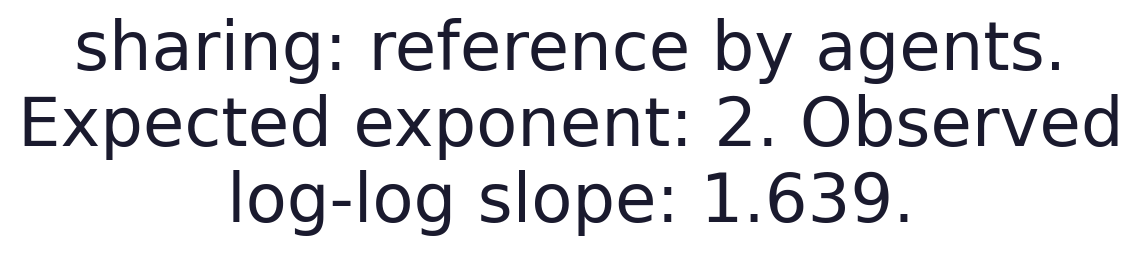
\includegraphics[keepaspectratio,width=0.98\linewidth,height=0.8\textheight,alt={sharing: reference by agents. Expected exponent: 2. Observed log-log slope: 1.639.}]{../figures/complexity_scaling.slide-group-2-share-round-naive-guide.png}
\refstepcounter{figure}\label{fig:complexity-scaling-slide-panel-8}
\end{figure}
\end{frame}

\begin{frame}{Computational complexity\ldots{} (part 27)}
\begin{figure}
\centering
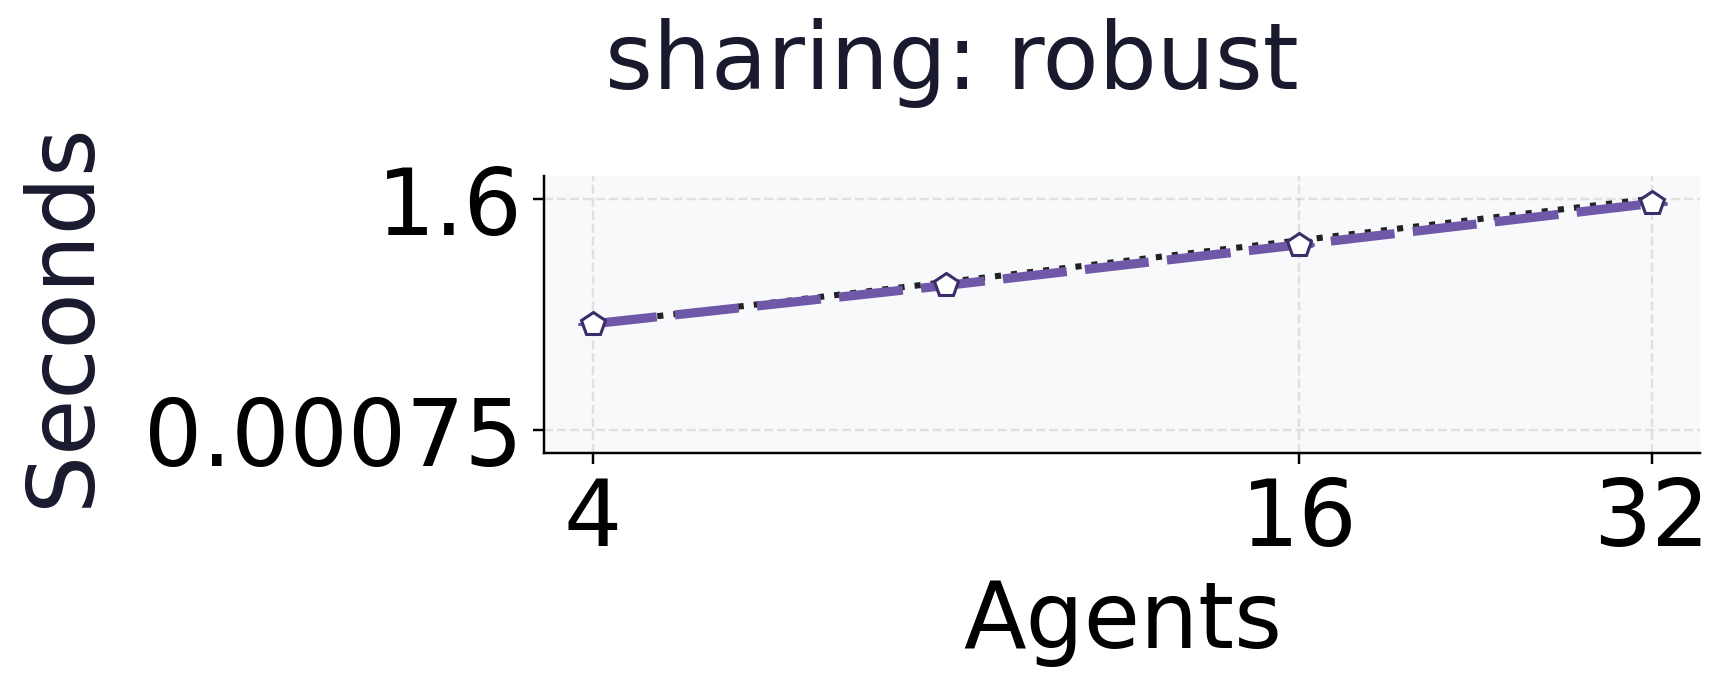
\includegraphics[keepaspectratio,width=0.98\linewidth,height=0.8\textheight,alt={share\_round\_robust by agents: all measured medians, observed min-max ranges and normalized expected-exponent guide on common group scales.}]{../figures/complexity_scaling.slide-group-2-share-round-robust.png}
\refstepcounter{figure}\label{fig:complexity-scaling-slide-panel-9}
\end{figure}
\end{frame}

\begin{frame}{Computational complexity\ldots{} (part 28)}
\begin{figure}
\centering
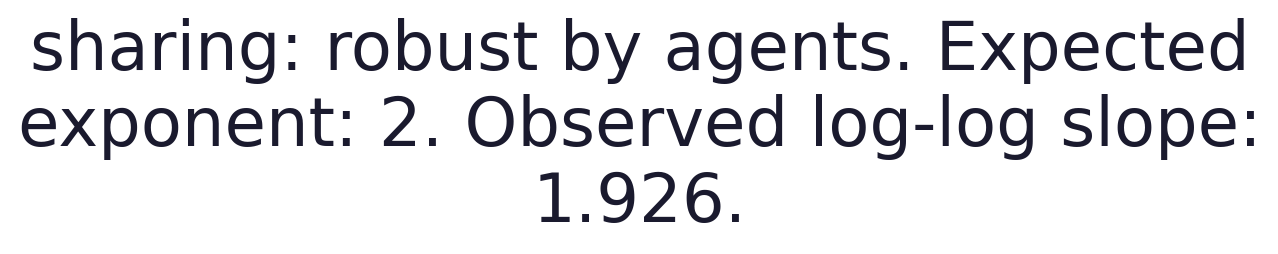
\includegraphics[keepaspectratio,width=0.98\linewidth,height=0.8\textheight,alt={sharing: robust by agents. Expected exponent: 2. Observed log-log slope: 1.926.}]{../figures/complexity_scaling.slide-group-2-share-round-robust-guide.png}
\refstepcounter{figure}\label{fig:complexity-scaling-slide-panel-10}
\end{figure}
\end{frame}

\begin{frame}{Computational complexity\ldots{} (part 29)}
\begin{figure}
\centering
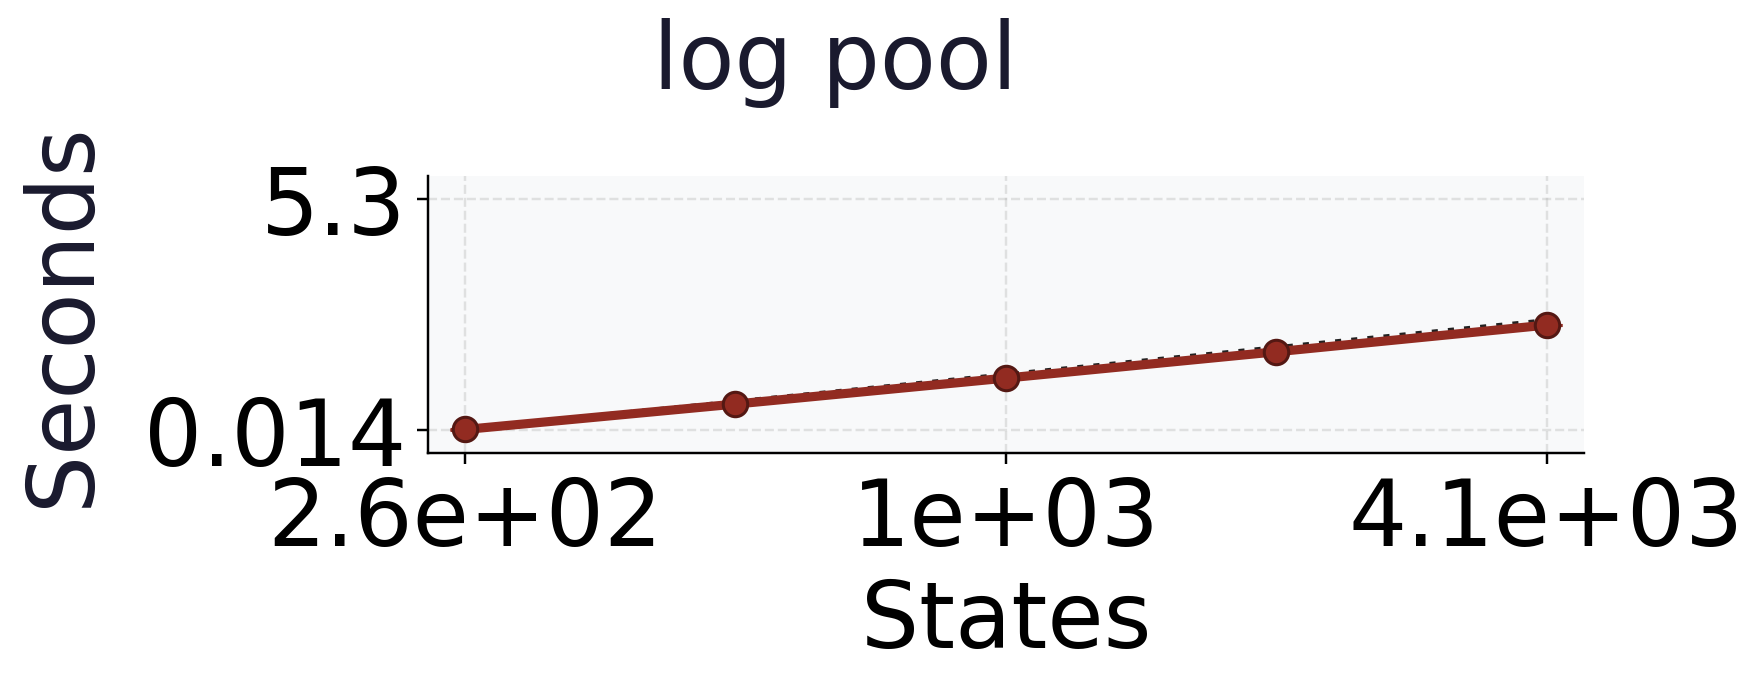
\includegraphics[keepaspectratio,width=0.98\linewidth,height=0.8\textheight,alt={log\_linear\_pool by states: all measured medians, observed min-max ranges and normalized expected-exponent guide on common group scales.}]{../figures/complexity_scaling.slide-group-3-log-linear-pool.png}
\refstepcounter{figure}\label{fig:complexity-scaling-slide-panel-11}
\end{figure}
\end{frame}

\begin{frame}{Computational complexity\ldots{} (part 30)}
\begin{figure}
\centering
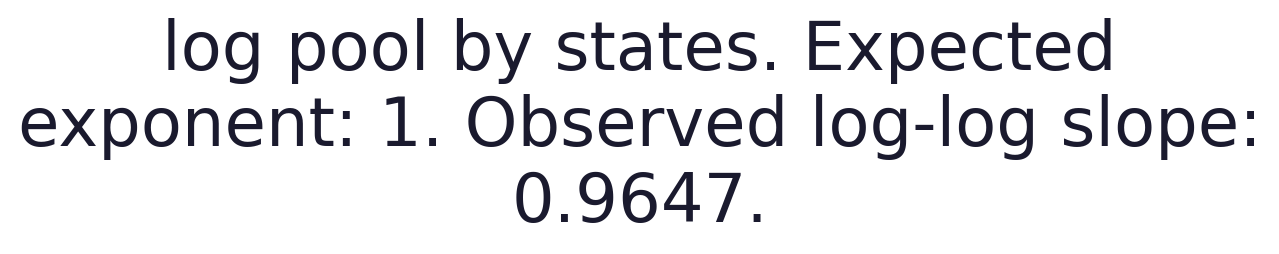
\includegraphics[keepaspectratio,width=0.98\linewidth,height=0.8\textheight,alt={log pool by states. Expected exponent: 1. Observed log-log slope: 0.9647.}]{../figures/complexity_scaling.slide-group-3-log-linear-pool-guide.png}
\refstepcounter{figure}\label{fig:complexity-scaling-slide-panel-12}
\end{figure}
\end{frame}

\begin{frame}{Computational complexity\ldots{} (part 31)}
\begin{figure}
\centering
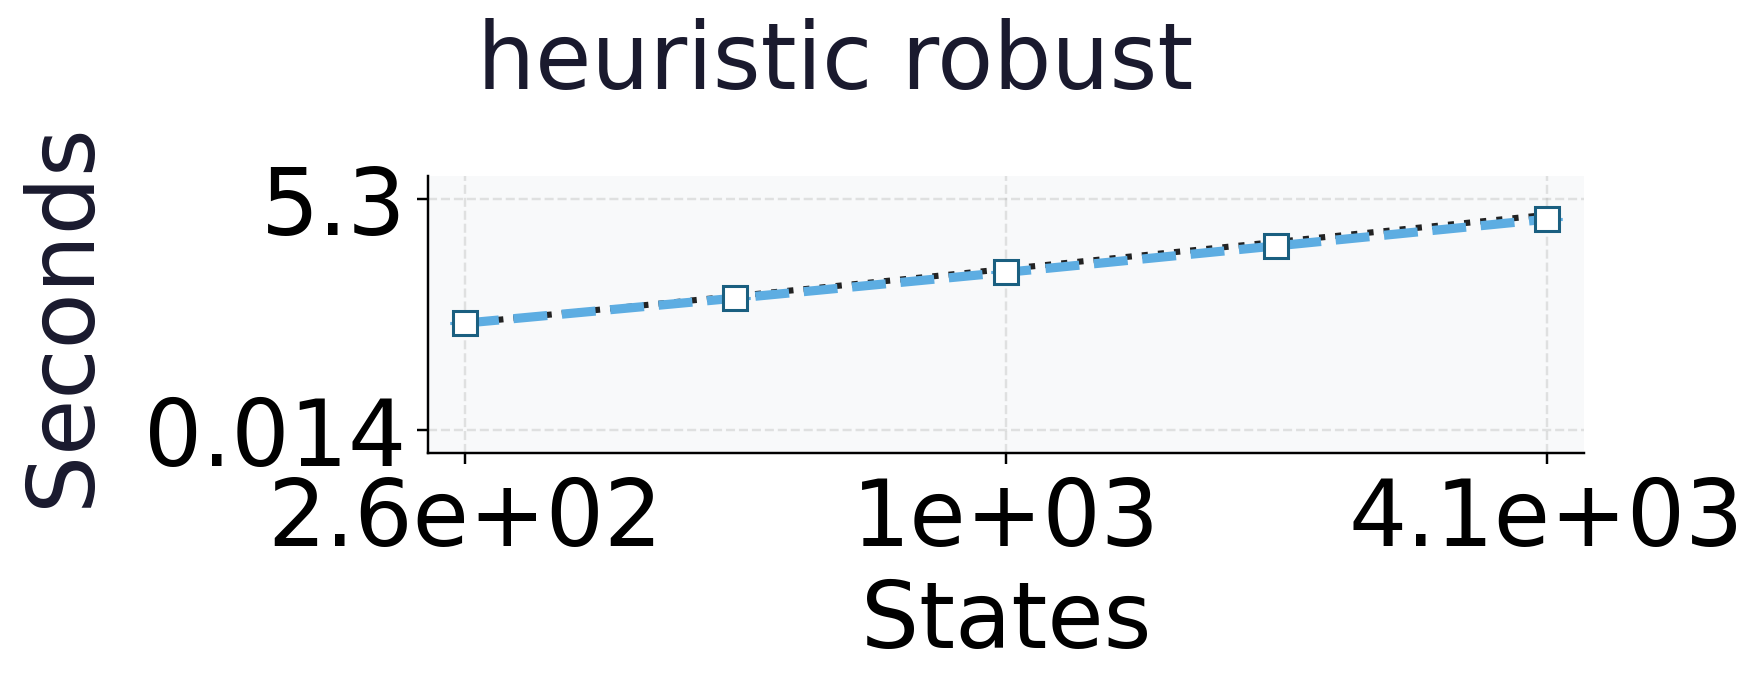
\includegraphics[keepaspectratio,width=0.98\linewidth,height=0.8\textheight,alt={robust\_aggregate by states: all measured medians, observed min-max ranges and normalized expected-exponent guide on common group scales.}]{../figures/complexity_scaling.slide-group-3-robust-aggregate.png}
\refstepcounter{figure}\label{fig:complexity-scaling-slide-panel-13}
\end{figure}
\end{frame}

\begin{frame}{Computational complexity\ldots{} (part 32)}
\begin{figure}
\centering
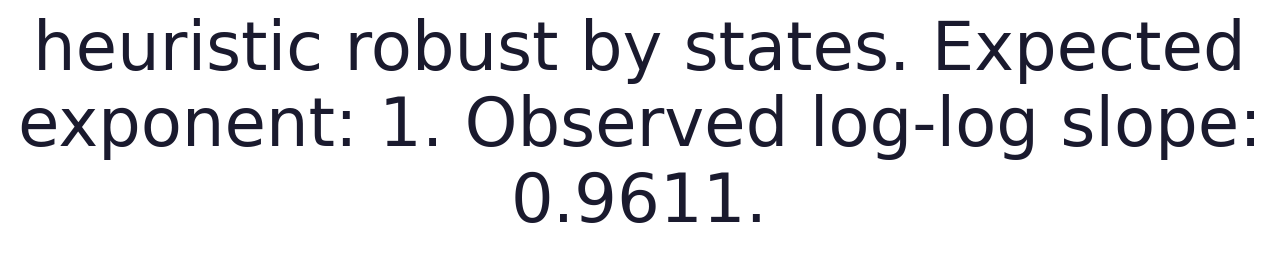
\includegraphics[keepaspectratio,width=0.98\linewidth,height=0.8\textheight,alt={heuristic robust by states. Expected exponent: 1. Observed log-log slope: 0.9611.}]{../figures/complexity_scaling.slide-group-3-robust-aggregate-guide.png}
\refstepcounter{figure}\label{fig:complexity-scaling-slide-panel-14}
\end{figure}
\end{frame}

\begin{frame}{Computational complexity\ldots{} (part 33)}
\begin{figure}
\centering
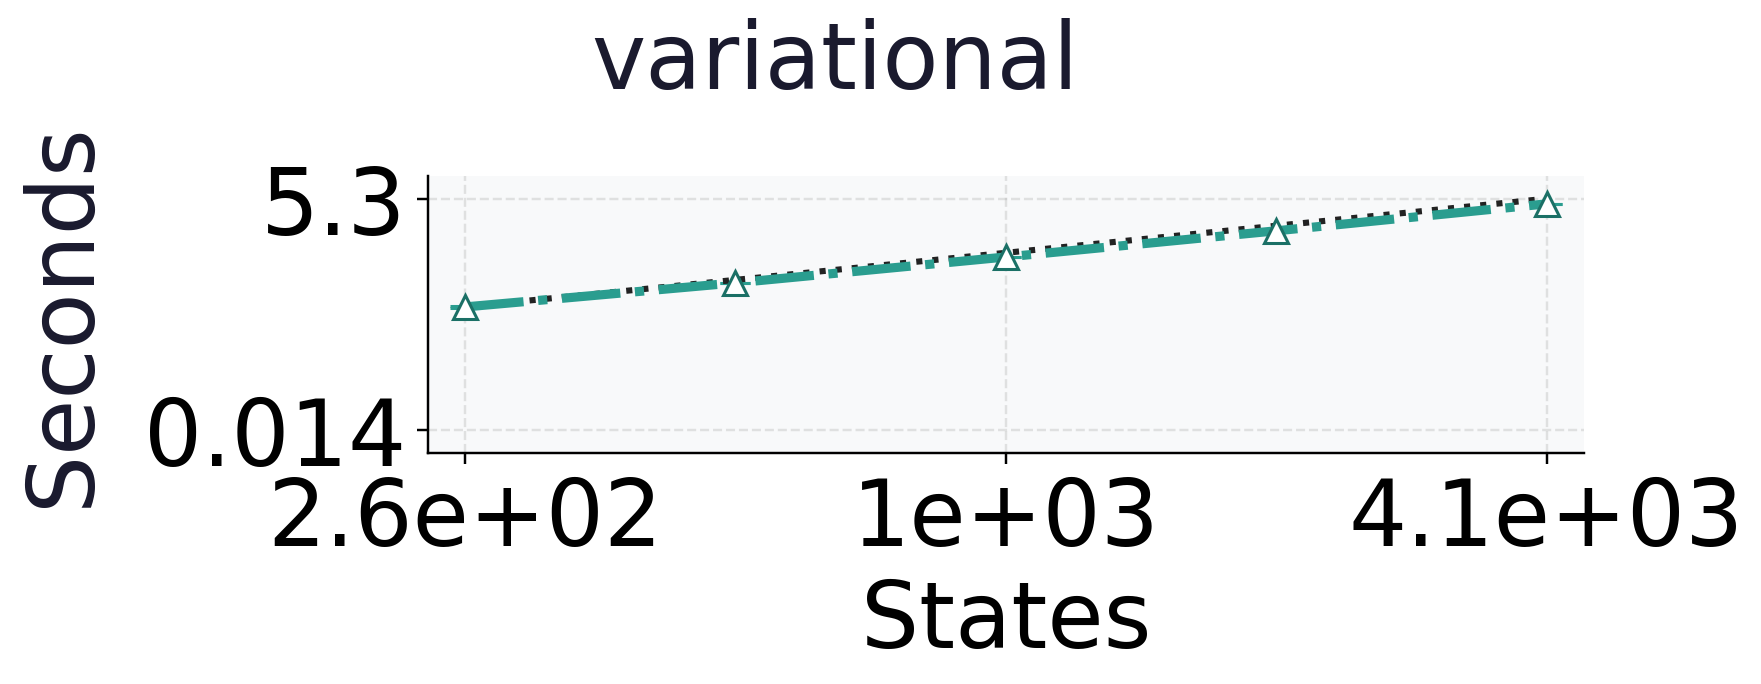
\includegraphics[keepaspectratio,width=0.98\linewidth,height=0.8\textheight,alt={variational\_aggregate by states: all measured medians, observed min-max ranges and normalized expected-exponent guide on common group scales.}]{../figures/complexity_scaling.slide-group-3-variational-aggregate.png}
\refstepcounter{figure}\label{fig:complexity-scaling-slide-panel-15}
\end{figure}
\end{frame}

\begin{frame}{Computational complexity\ldots{} (part 34)}
\begin{figure}
\centering
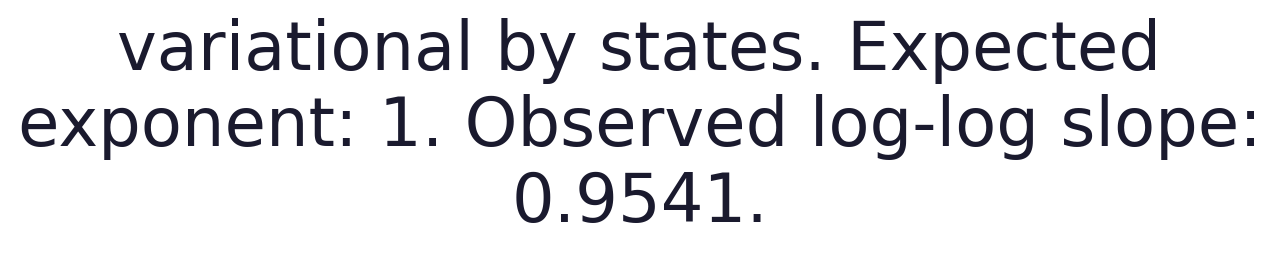
\includegraphics[keepaspectratio,width=0.98\linewidth,height=0.8\textheight,alt={variational by states. Expected exponent: 1. Observed log-log slope: 0.9541.}]{../figures/complexity_scaling.slide-group-3-variational-aggregate-guide.png}
\refstepcounter{figure}\label{fig:complexity-scaling-slide-panel-16}
\end{figure}
\end{frame}

\begin{frame}{Computational complexity\ldots{} (part 35)}
\begin{figure}
\centering
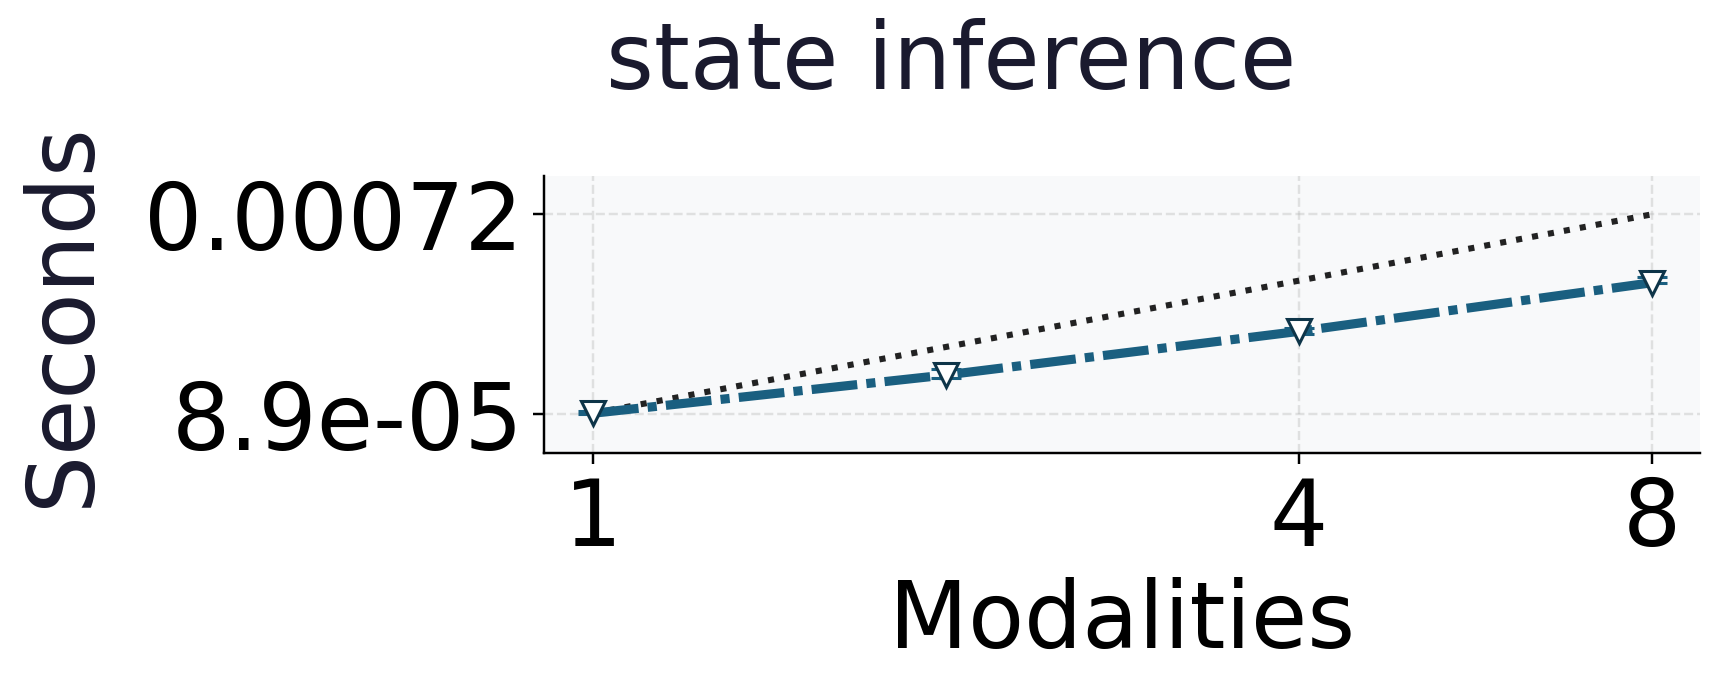
\includegraphics[keepaspectratio,width=0.98\linewidth,height=0.8\textheight,alt={infer\_states by modalities: all measured medians, observed min-max ranges and normalized expected-exponent guide on common group scales.}]{../figures/complexity_scaling.slide-group-4-infer-states.png}
\refstepcounter{figure}\label{fig:complexity-scaling-slide-panel-17}
\end{figure}
\end{frame}

\begin{frame}{Computational complexity\ldots{} (part 36)}
\begin{figure}
\centering
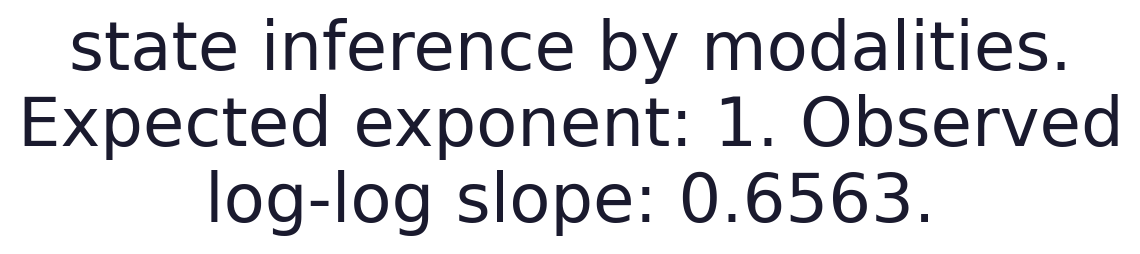
\includegraphics[keepaspectratio,width=0.98\linewidth,height=0.8\textheight,alt={state inference by modalities. Expected exponent: 1. Observed log-log slope: 0.6563.}]{../figures/complexity_scaling.slide-group-4-infer-states-guide.png}
\refstepcounter{figure}\label{fig:complexity-scaling-slide-panel-18}
\end{figure}
\end{frame}

\begin{frame}{Computational complexity\ldots{} (part 37)}
\begin{figure}
\centering
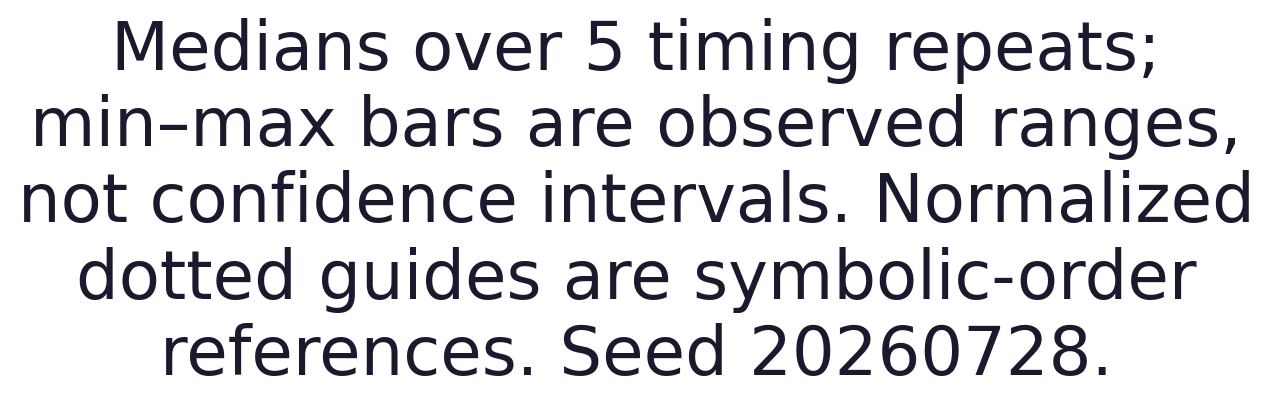
\includegraphics[keepaspectratio,width=0.98\linewidth,height=0.8\textheight,alt={Medians over 5 timing repeats; min--max bars are observed ranges, not confidence intervals. Normalized dotted guides are symbolic-order references. Seed 20260728.}]{../figures/complexity_scaling.slide-scope.png}
\refstepcounter{figure}\label{fig:complexity-scaling-slide-panel-19}
\end{figure}
\end{frame}

\end{document}
